\chapter{Methodology}
\label{Ch:methodology}
\chapterprecis{
In this chapter the theoretical background developed in \autoref{Ch:Theory}  will
be put to practice to solve an actual example problem. This chapter will
explain the problem that is to be solved. It will explain how the model
is set up for aeroelastic analysis as well as the process used to
optimize the design.}

\section{Problem Introduction }
\label{problem-introduction}

The problem that has been chosen as an example application of all the
theory developed in the previous chapter is the flutter characteristics
study of the ASW 28 glider main wing and the subsequent material design
optimization to tailor the flutter characteristics to specific
requirements. This choice of this specific aircraft is because it has an
extremely large aspect ratio thus making it also very flexible.
Moreover, the main goal of a glider is to achieve the best glide angle
so reduction of weight is of utmost importance and so these vehicles are
ideal for this application as they combine the high likelihood of
flutter occurring with the need to optimize for the lowest weight
possible.

''The ASW 28 is Schleicher's high-performance glider for the
FAI-Standard Class with 15m span.'' \cite{asw28}. The technical data of this
aircraft are summarized in \autoref{fig:TechnicalDataofASW28glider} :

\begin{figure}[H]
\centering
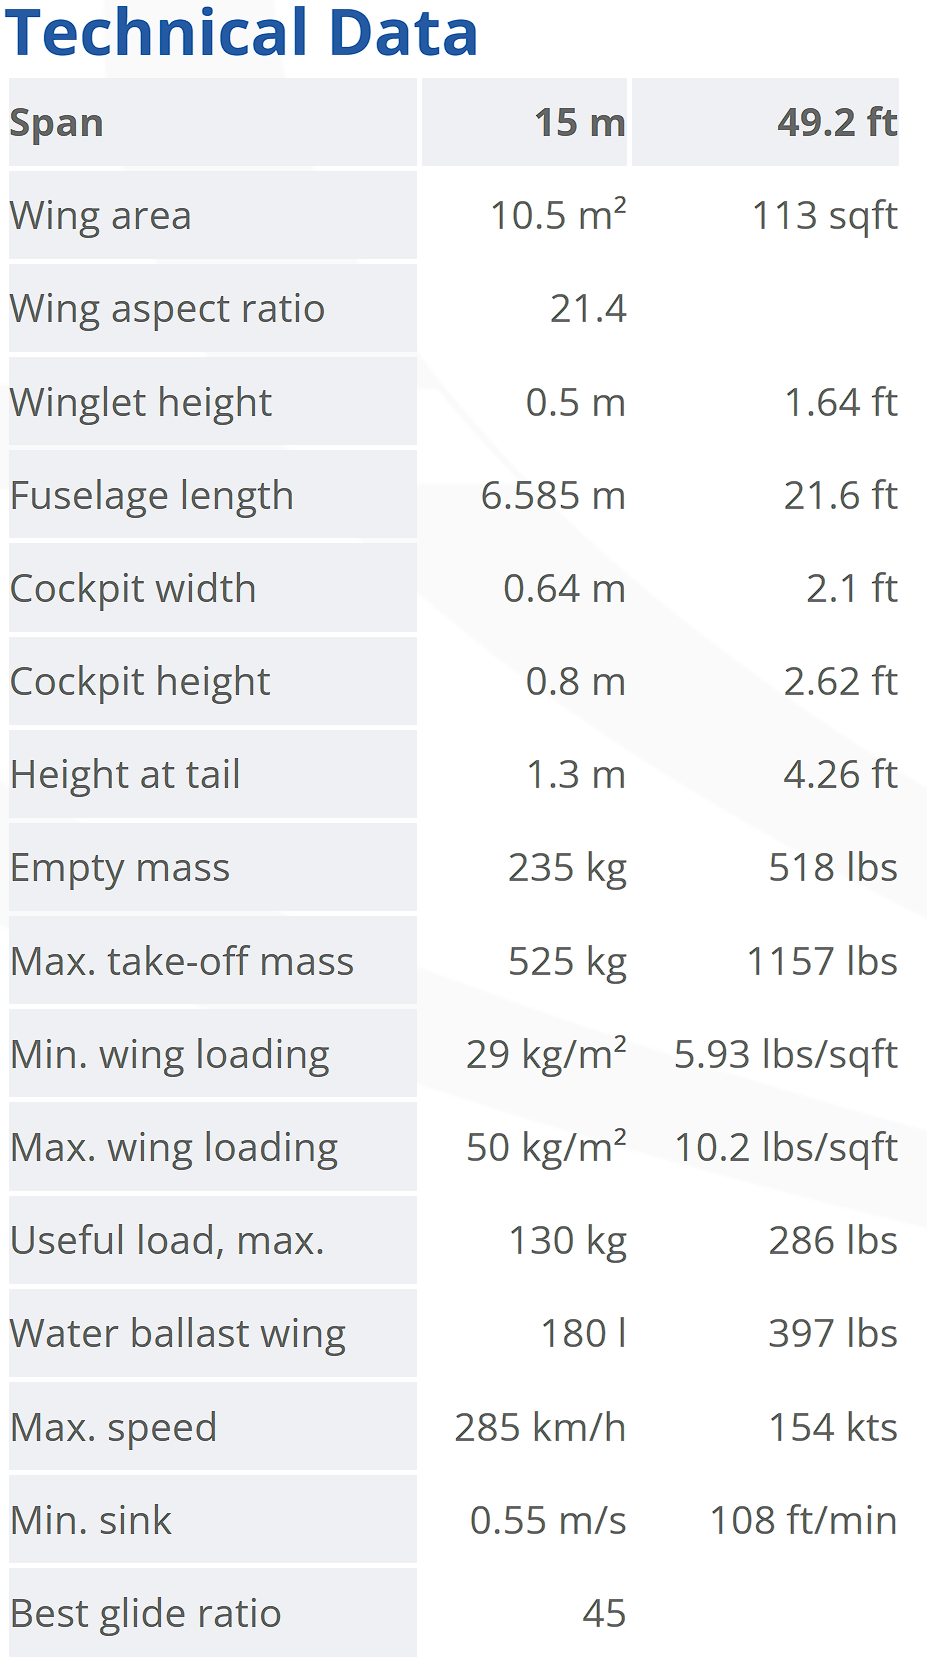
\includegraphics[width=2.92073in]{ASW28_characteristics.png}
\caption{Technical Data of ASW 28 glider \cite{asw28}}
\label{fig:TechnicalDataofASW28glider}
\end{figure}

\begin{figure}[H]
\centering
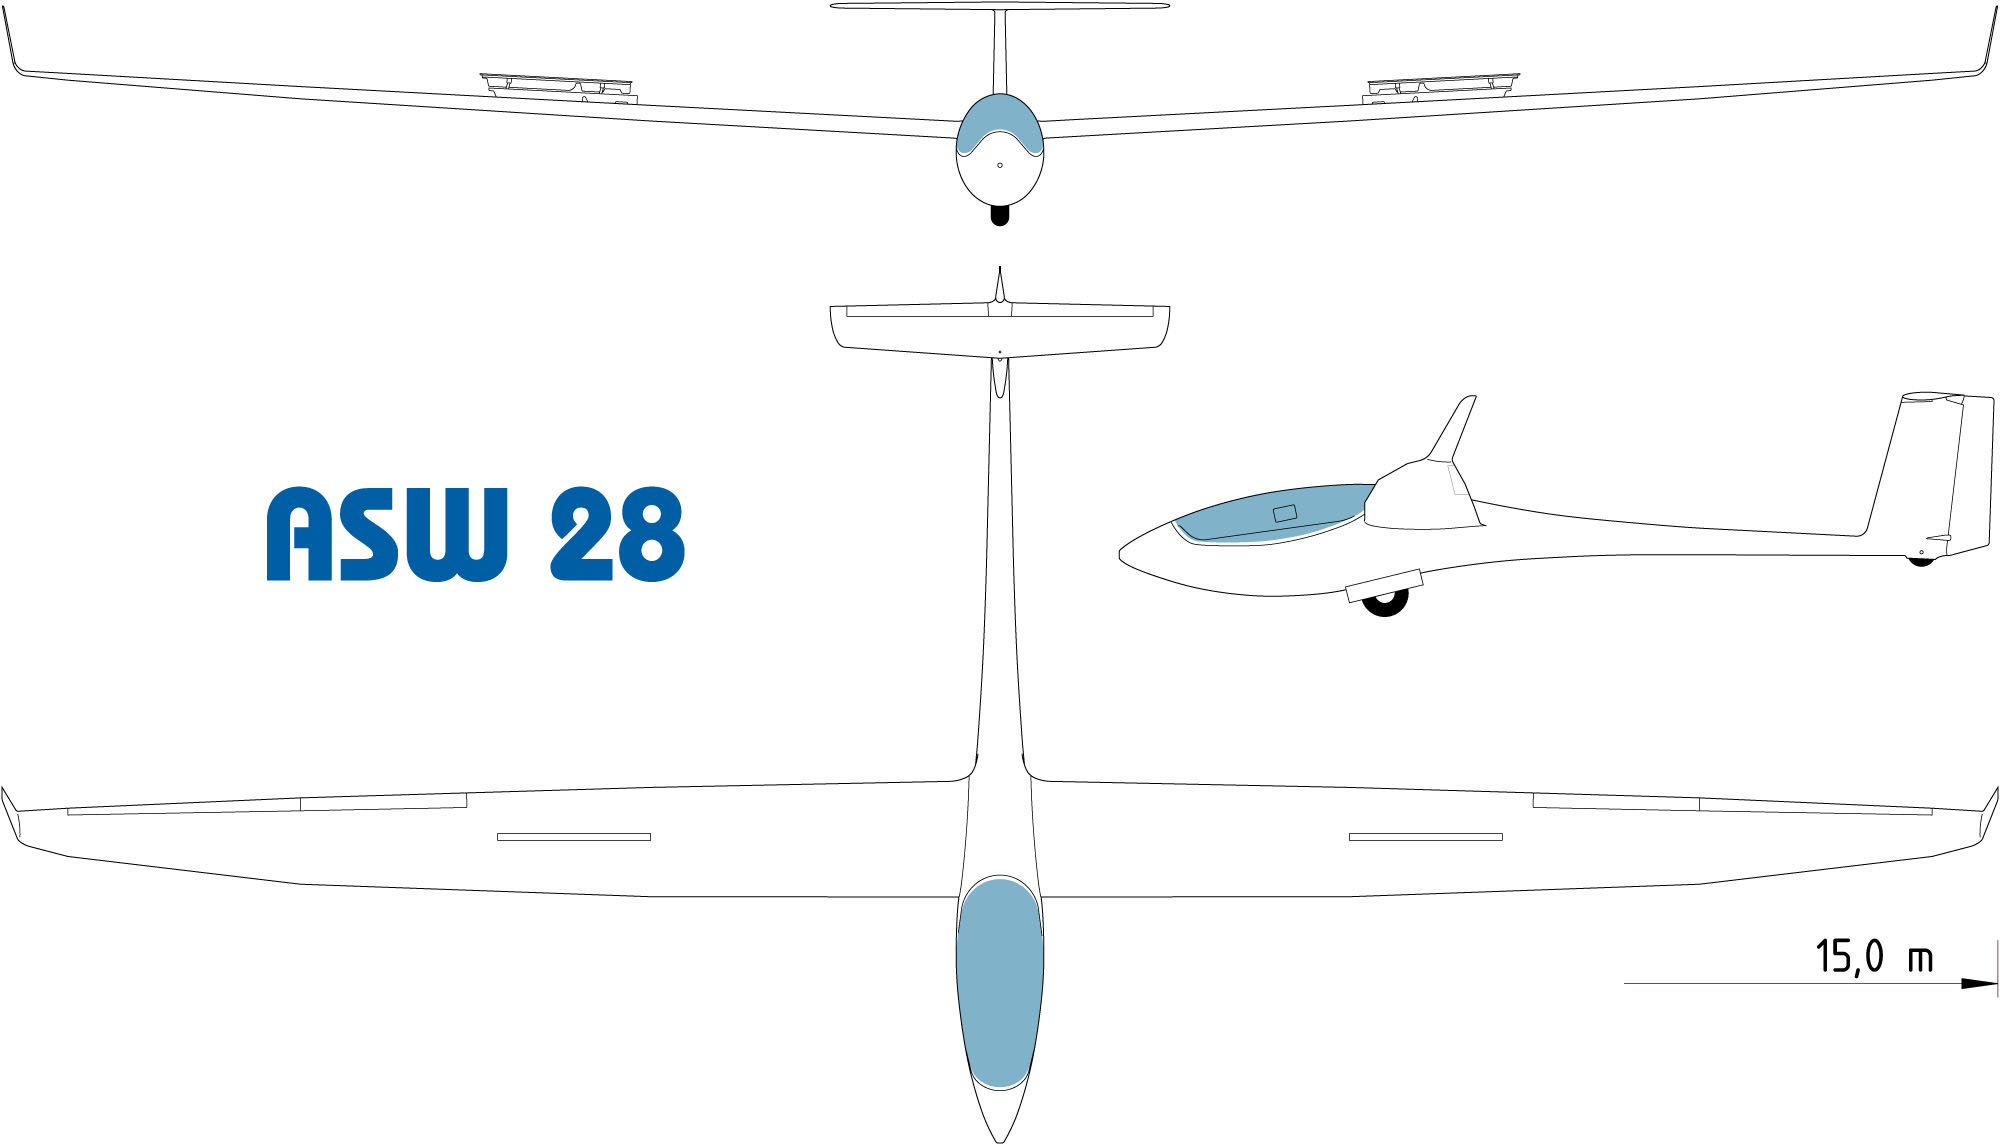
\includegraphics[width=5.5026in,height=3.34935in]{ASW 28 3side view.png}
\caption{Front, side and top view of ASW 28 glider \cite{asw28}}
\end{figure}

The analysis of the main Wing of the ASW 28 will include the following
steps:

\begin{enumerate}
\def\labelenumi{\arabic{enumi}.}
\item
  Model set up in Altair HyperMesh for modal analysis and flutter
  analysis
\item
  Creation of a Python script to read Flutter results from Optistruct
  solver
\item
  Definition of Optimization problem parameters using different
  optimization techniques and implementation using Python.
\end{enumerate}

\section{ASW 28 main Composite Wing Model}
\label{asw-28-main-composite-wing-model}

\subsection{Wing Geometry \&
Discretization}\label{wing-geometry-discretization}

The external geometry of the Wing was imported to HyperMesh from a CAD
file. The geometry was cleaned up so as to contain only the main wing of
the aircraft and because of some inaccuracies and the
non-metric length units used, a scale transformation had to be used.

\begin{figure}[H]
    \centering
    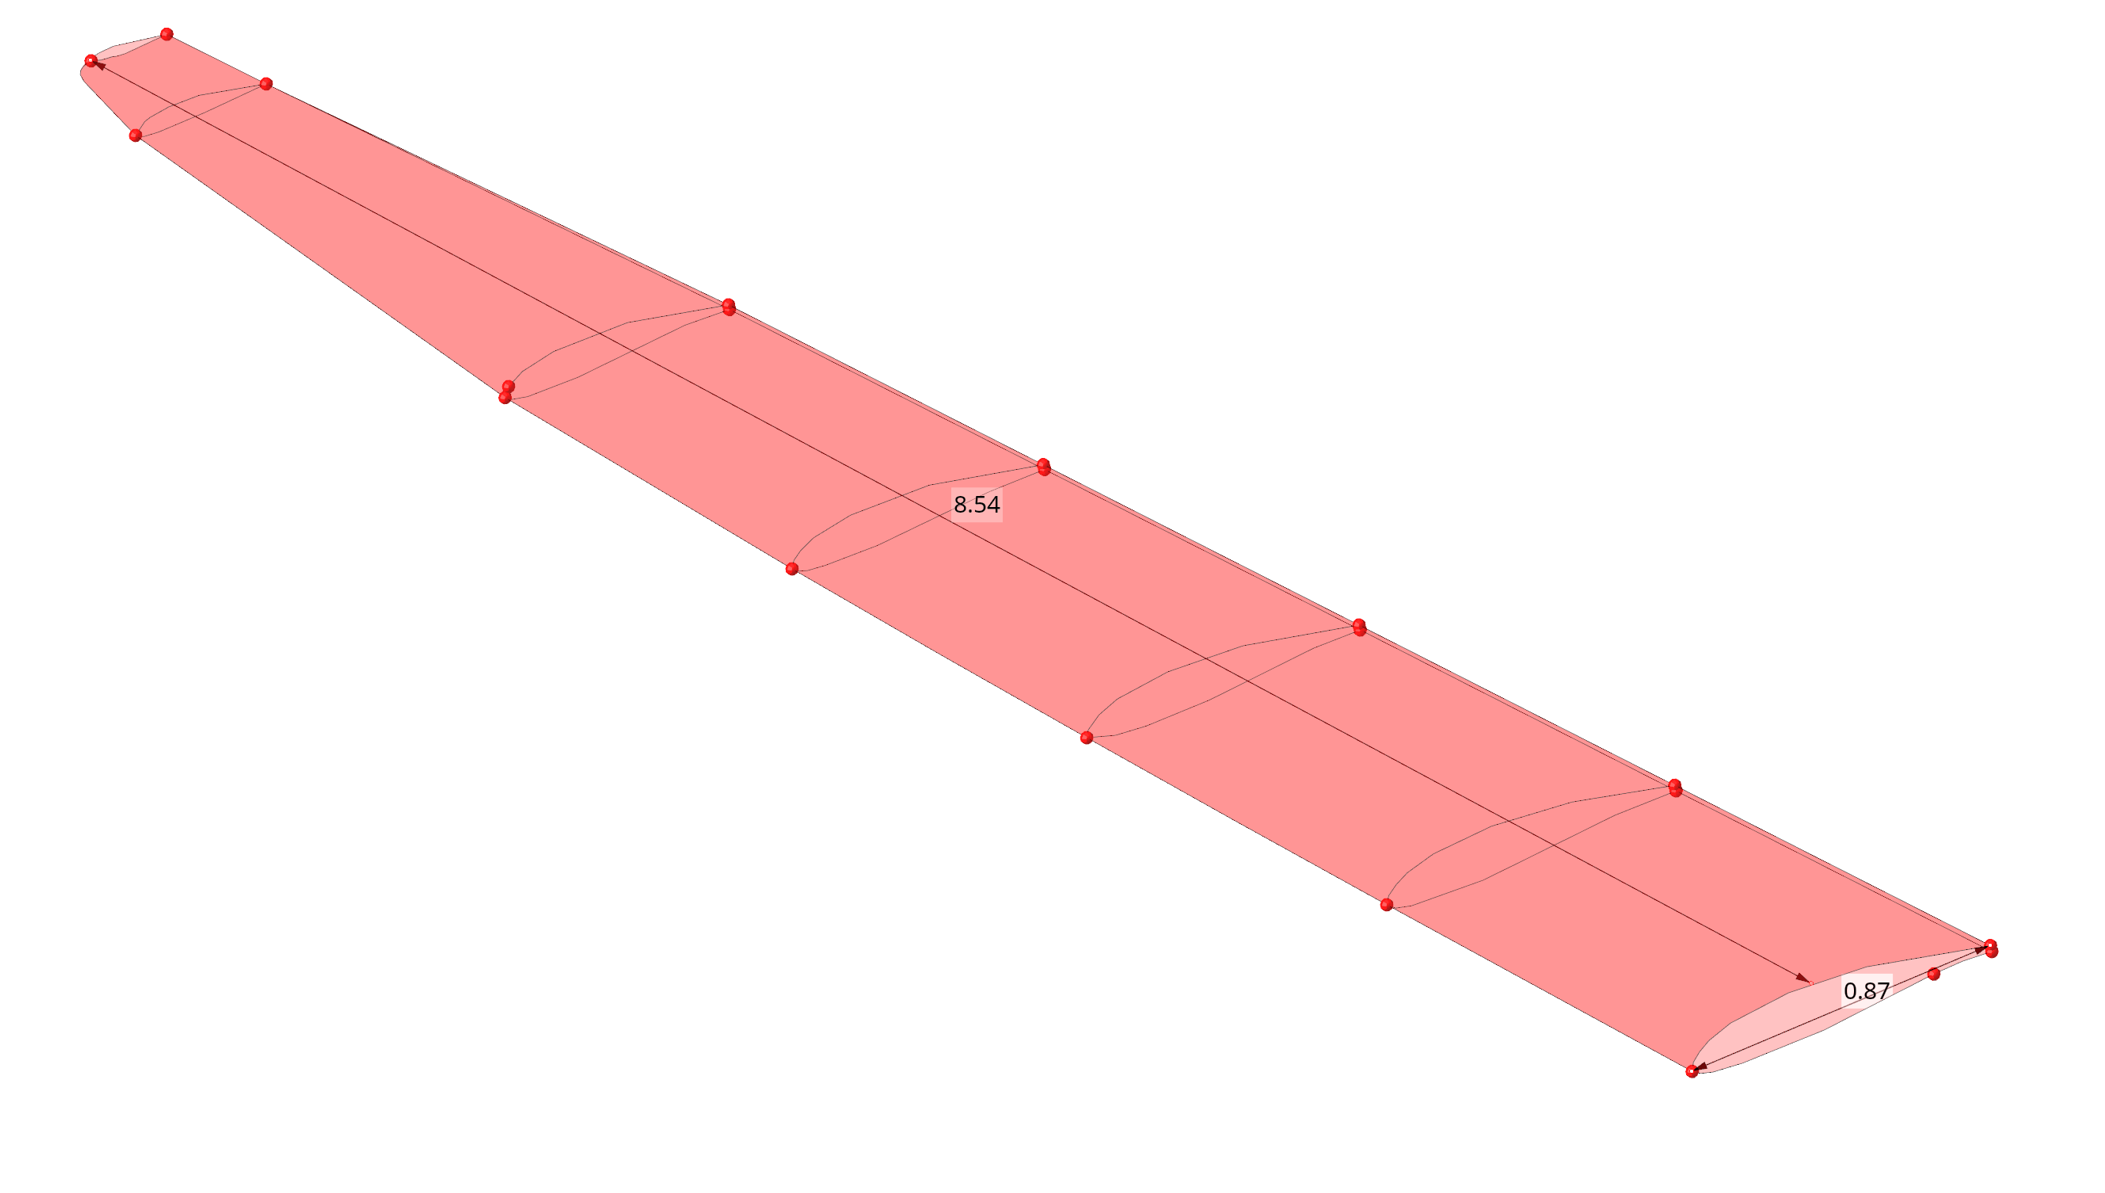
\includegraphics[width=\textwidth]{ASW 28 External Geometry.png}
    \caption{ASW 28 Wing external geometry (length in meters)}
\end{figure}

After the creation of the external geometry the internal structure of
the Wing had to be created from scratch. Since the detailed drawings of
the internal structure are not available, the internal structure
geometry was improvised based on some pictures of the disassembled wing.
The main features of most modern wings' internal geometry are the spars
and ribs. Spars are the main structural member of the wing which run
spanwise along the length of the wing and are responsible for carrying
aerodynamic loads to the main fuselage. Ribs are structural members of
the wing that run chordwise (perpendicular to the spars) and their
purpose is to support the wing's skin so that it maintains the proper
airfoil profile.

Modern glider wings usually have only one main spar and several ribs.
For this application a single main spar of rectangular cross section
which tapers towards the wing's tip and 6 ribs are used.

\begin{figure}[H]
    \centering
    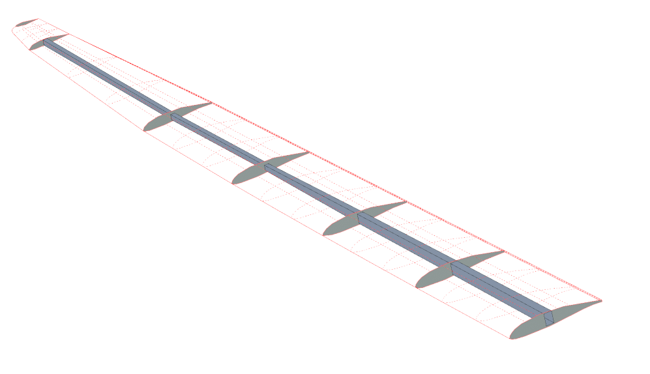
\includegraphics[width=\textwidth]{ASW 28 Internal Geometry.png}
    \caption{ASW 28 Wing Internal geometry}
\end{figure}


The discretization of the geometry was achieved using shell elements
arranged in a mesh which was created with the help of the ``Panel Mesh''
utility of HyperMesh for the skin of the wing since this function is
especially well suited for this type of panel-like geometry, and the
``General 2D Mesh'' utility for the internal geometry. The average
element size has a side length of \(0.02\ [m] \).

The discretization does not need to be very accurate since for the
flutter analysis we only need to capture enough detail to describe the
first few eigenmodes accurately and we do not care about the exact
stresses at specific points within the structure.

\begin{figure}[H]
\centering
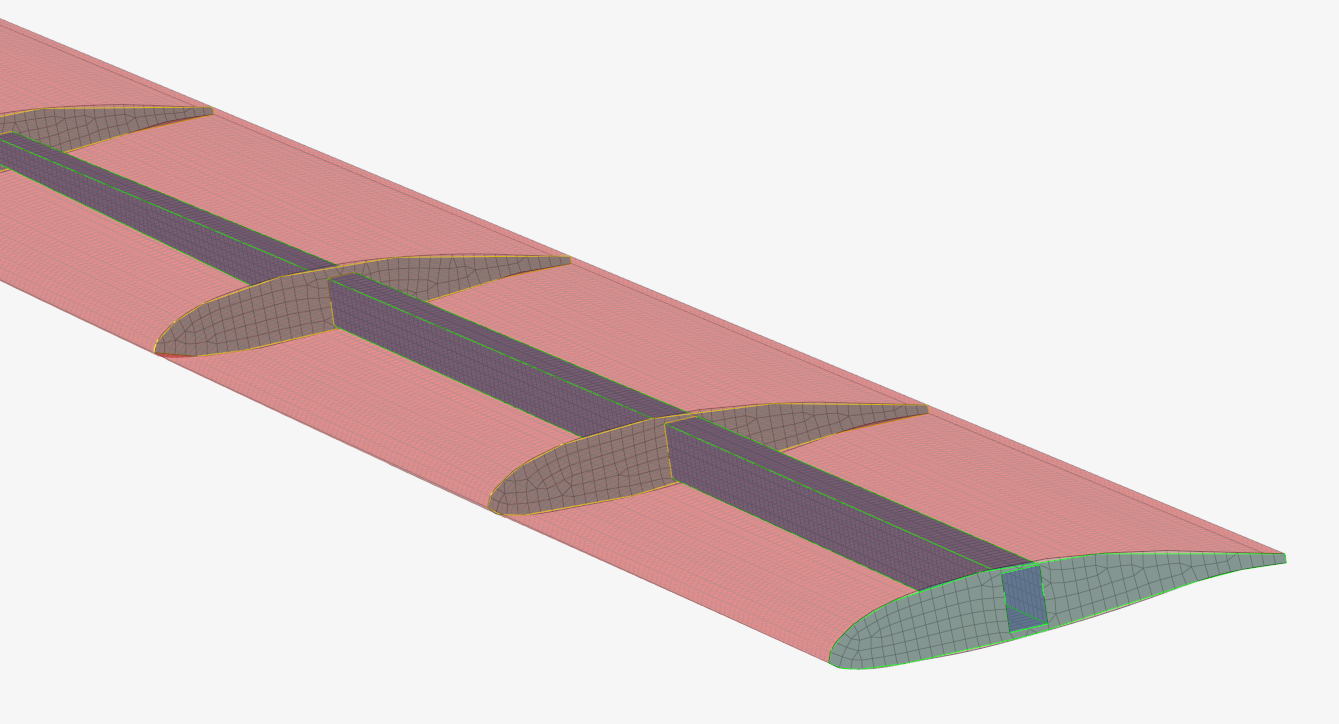
\includegraphics[width = \textwidth]{ASW 28 Wing Mesh.png}
\caption{ASW 28 Wing Internal mesh}
\end{figure}

\begin{figure}[H]
\centering
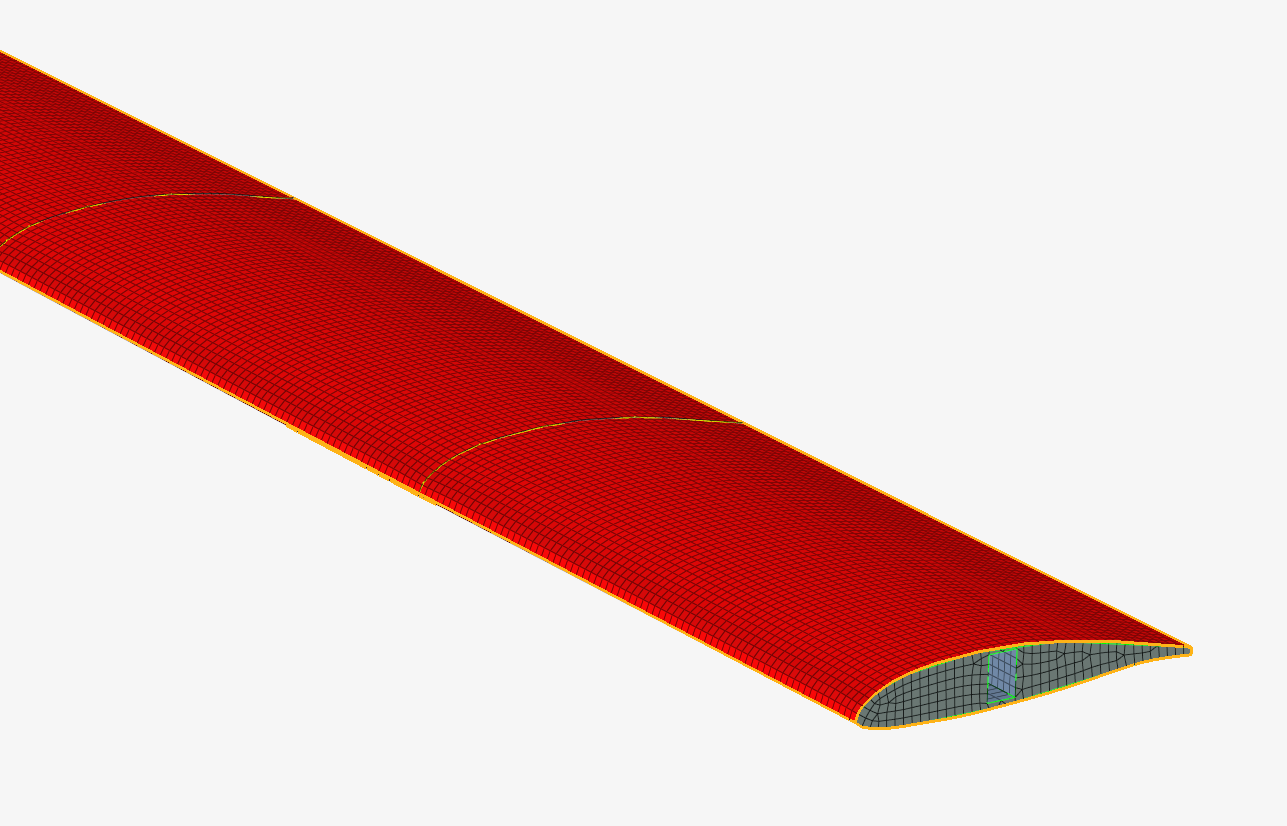
\includegraphics[width = \textwidth]{ASW 28 Wing Skin Mesh.png}
\caption{ASW 28 Wing skin mesh}
\end{figure}

\subsection{Material properties Definition}
\label{material-properties-definition.}

The material properties assigned to different components of the wing
structure are somewhat arbitrary as this information is not publicly
available. This should not pose any problems to the goal of this thesis
since during the optimization, material properties are subject to change
anyway.

A common composite material for the skin of high-performance gliders is
fiberglass or carbon fiber, because these materials offer high strength,
low weight and a smooth aerodynamic surface. For this application a
carbon fiber - Epoxy composite was chosen. For the Optistruct solver
this kind of composite material can be defined using the MAT8 material
card with the following properties \cite{matweb}:

\begin{itemize}
\item
  \(E_{1} = 125\ GPa\)
\item
  \(E_{2} = 8.41GPa\)
\item
  \(\nu_{12} = 0.35\)
\item
  \(G_{12} = 4.23\ GPa\)
\item
  \(\rho = 1517\ kg\text{/}m^{3}\)
\end{itemize}

This material is a laminated composite and although the material
properties have been sufficiently defined the laminate structure hasn't.
To define the laminate configuration a PCOMP property card is needed.
This card is essentially a list containing the properties of each
laminate layer. These properties are:

\begin{enumerate}
\def\labelenumi{\arabic{enumi}.}
\item
  The material of the laminate layer defined as a composite material
  card, in this case a MAT8 card
\item
  The thickness of each laminate layer defined as a float
\item
  The angle in degrees at which the primary axis (axis 1) of the
  laminate layer is oriented
\end{enumerate}

For this application a six-layer laminate composite will be created
using the carbon fiber epoxy orthotropic material with angles
alternating between +45 and -45 degrees and a thickness of \(0.5\ mm\)
for each layer.

For the internal structure of the wing an aviation grade aluminum is
used. More specifically aluminum 6061 is used, which has the following
properties:

\begin{itemize}
\item
  \(E = 69\ GPa\)
\item
  \(\nu = 0.33\)
\item
  \(\rho = 2700\ kg\text{/}m^{3}\)
\end{itemize}

This is an isotropic material and is defined within Optistruct with a
MAT1 card which essentially lists these material parameters in a
specific manner.

Similarly, the material definition alone is not enough as we are working
with shell elements, a property which defines the thickness of the
material need to be present. In Optistruct this property is defined
using a PSHELL property card which only needs to hold a material
reference and a thickness value. In this chase the thickness is uniform
everywhere and equal to \(t = 2mm\)

\subsection{Boundary Conditions} \label{boundary-conditions}

The boundary conditions defined for this problem are similar to that of
a fixed free cantilever beam. The nodes at the root of the wing are
fixed along every degree of freedom with an SPC (Single Point
Constraint) entry. These boundary conditions assume that the wing's root
is completely fixed on its support which works well for a detached wing
which is placed on a test bench but are only an approximation of the
real flight situation where the wing is fixed to the fuselage which is
not static during flight.

\begin{figure}[H]
\centering
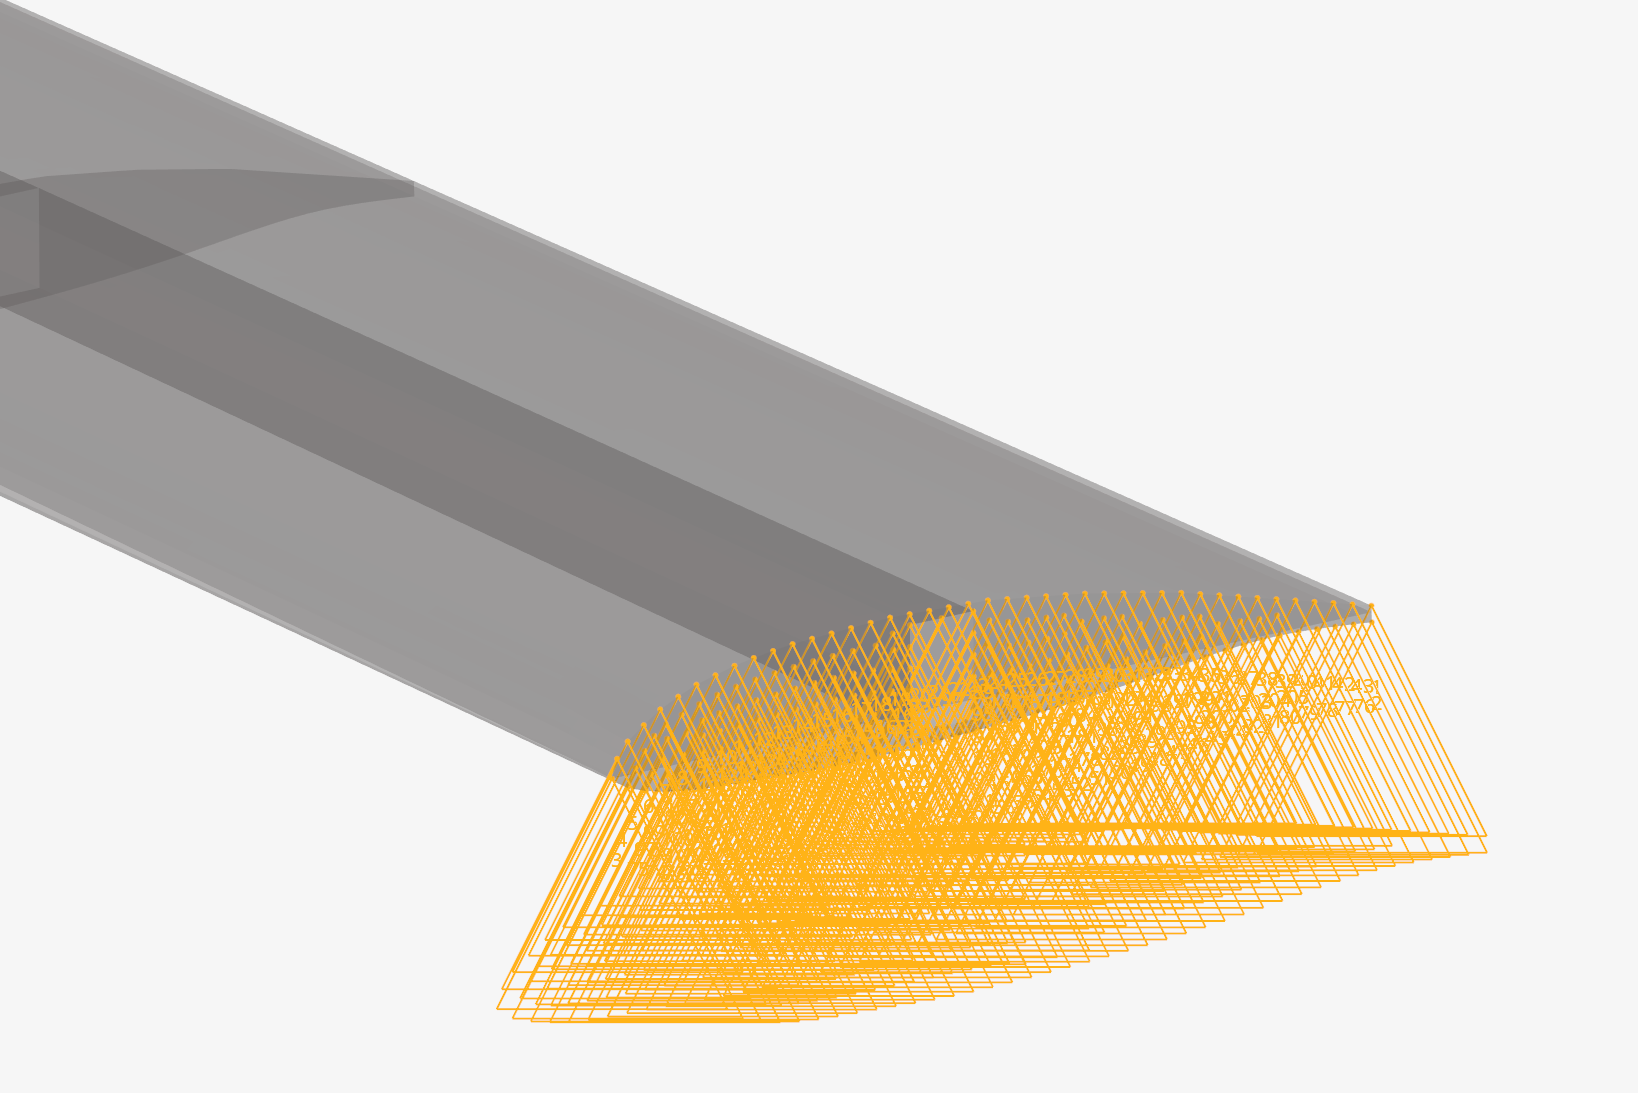
\includegraphics[width = \textwidth]{ASW 28 SPC.png}
\caption{ASW 28 Wing Boundary conditions}
\end{figure}

\subsection{Aerodynamic Grid}
\label{aerodynamic-grid}

To create the vortex-lattice the lifting surface of the wing needs to be
discretized. The way this is modeled in Optistruct is through the CAERO1
card which defines an ``aerodynamic macro element'' with a simple
two-dimensional quadrilateral geometry which is split into a predefined
number of boxes in the chordwise and spanwise directions. To define the
CAERO1 card one must first define the four corner points in a specified
order:

\begin{itemize}
\item
  The first point is on the leading edge and on the root of the wing
\item
  The second point has the same y coordinate as the first but lies on
  the trailing edge of the wing
\item
  The third point lies on the tip of the wing and at the trailing edge
\item
  The Fourth point has the same Y coordinate as the third but lies on
  the leading edge of the tip of the wing
\end{itemize}

\begin{figure}[H]
    \centering
    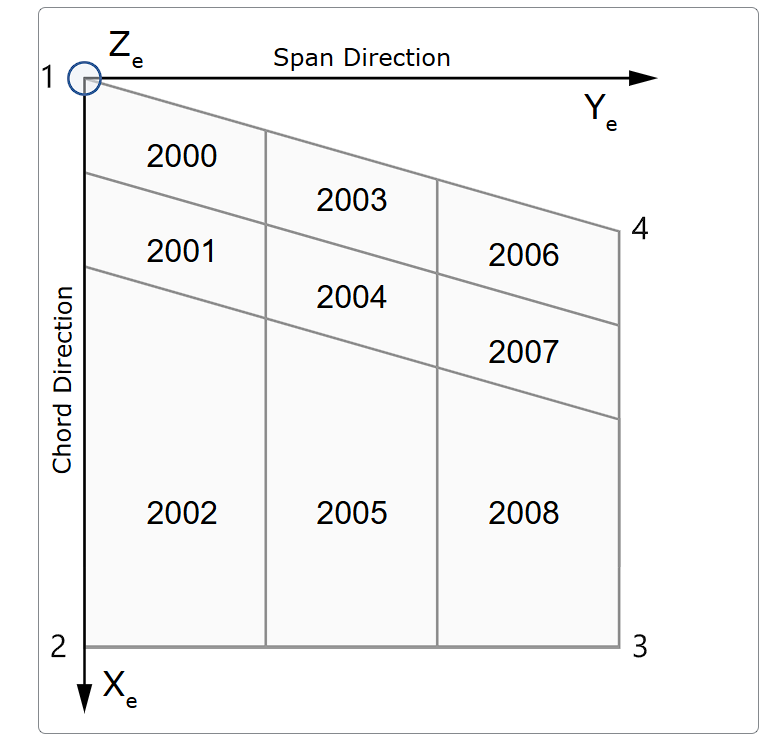
\includegraphics[width=0.6\textwidth]{CAERO1 Coordinate system.png}
    \caption{Coordinate System of CAERO1 Aerodynamic panel \cite{altair_flutter_tips}}
\end{figure}


This allows for the modelling of only simple trapezoidal geometries.
Since the projection of the ASW28 glider wing on the XY plane does not
fit well within a single trapezoidal shape two of these macro elements
were used to capture the variable taper ration of this wing. These
panels can be seen in the following image of the model.

\begin{figure}[H]
\centering
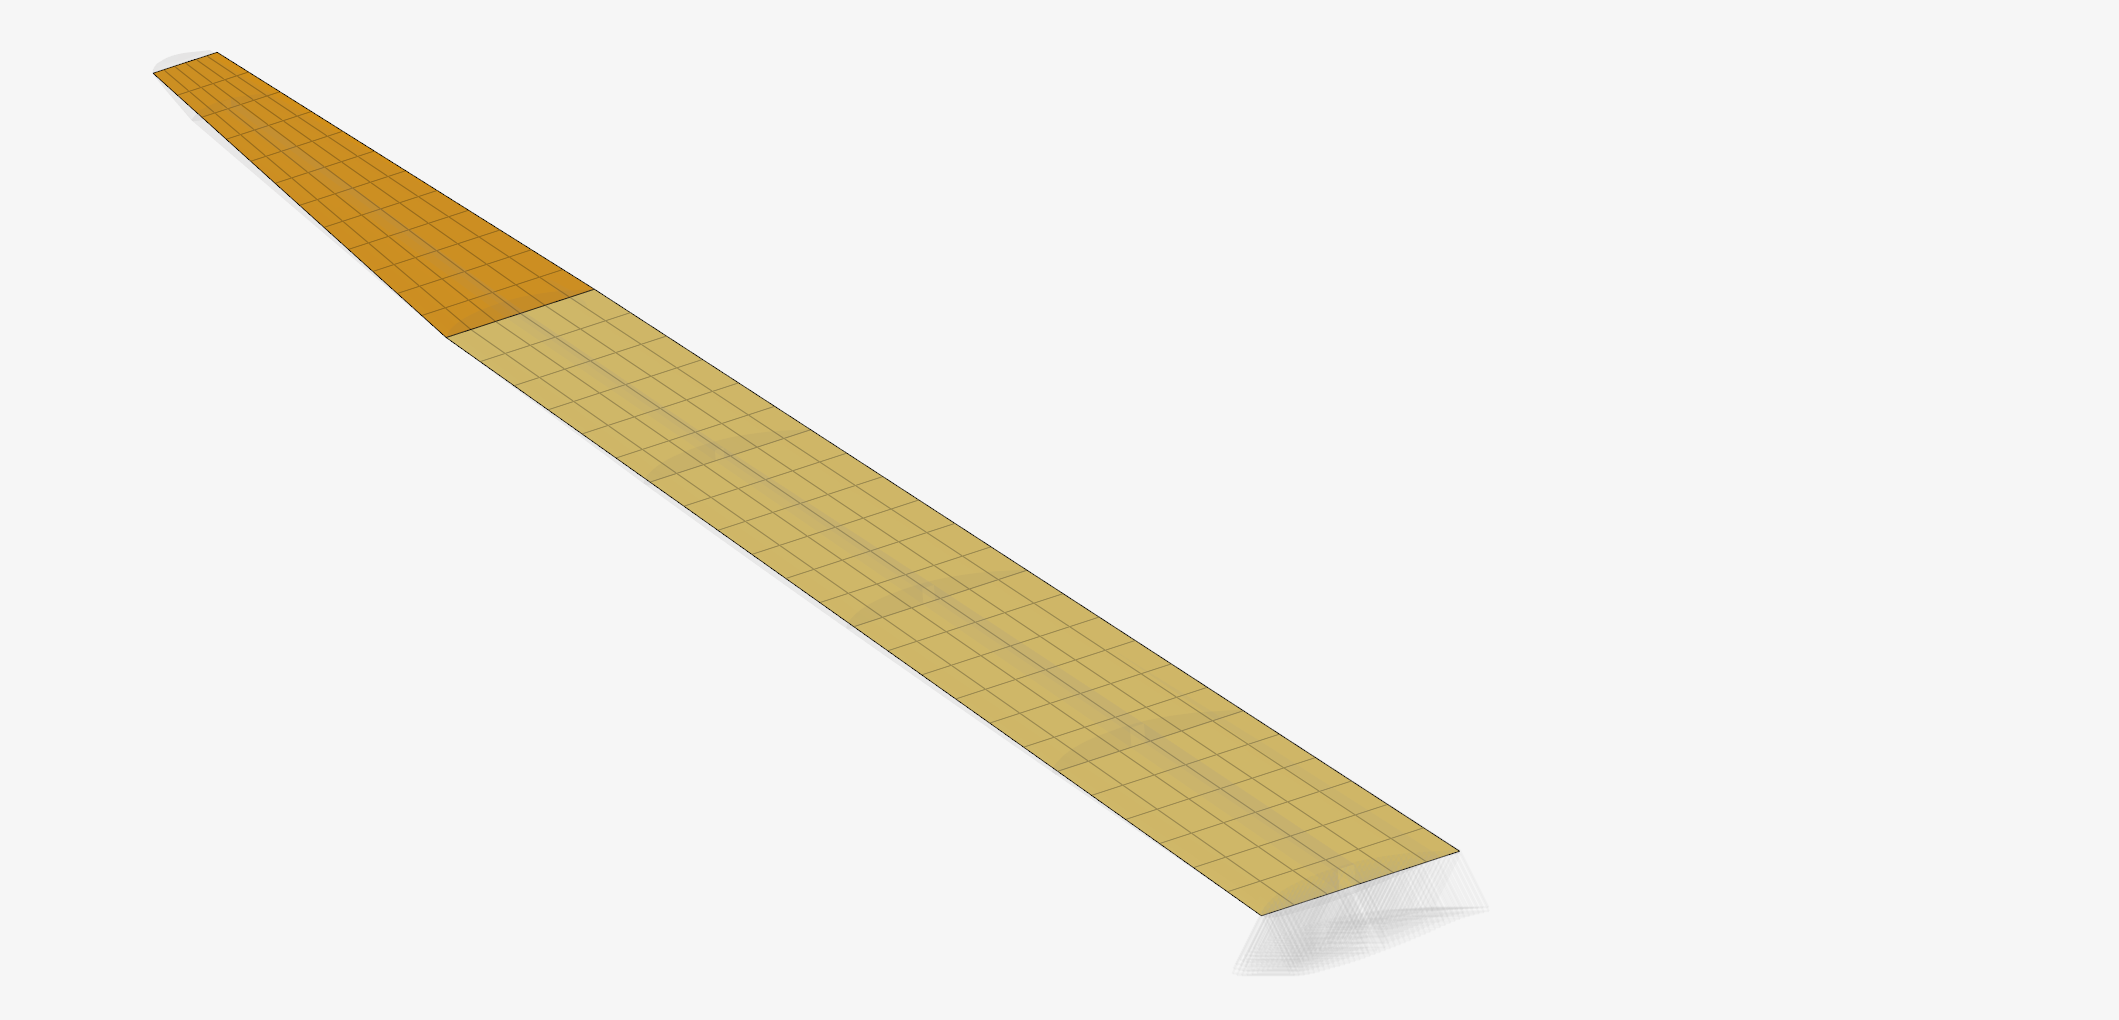
\includegraphics[width=4.65278in,height=3.01736in]{ASW 28 Aerodynamic grid.png}
\caption{CAERO1 macro elements of the ASW 28 Wing Model}
\end{figure}

The next step of defining the CAERO1 elements is defining the
discretization into aerodynamic boxes through two integer values NSAPN
and NCHORD which define the number of spanwise and chordwise boxes
respectively.

For the Inner CAERO1 macro element:

\[NSPAN = 24,\ \ NCHORD = 6\]

For the Outer CAERO1 macro element:

\[NSPAN = 12,\ \ NCHORD = 6\]

This discretization is chosen so that the aspect ratio of the boxes is
less than about three and the chordwise length of each box is less than
\(\Delta x < 0.08V_{\max}\ \text{/}f_{\max} \approx 0.65m\). These two
suggestions for the discretization of the aerodynamic panels are
specified in \cite{msc2021}

\subsection{The Spline}\label{the-spline}

In Flutter analysis the SPLINE entry is used to couple the structural
and aeroelastic domains. For this application a SPLINE1 entry is used
which defines a surface spline (linear splines are also available but do
not apply in this case.) To define the SPLINE1 the following entries are
needed:

\begin{itemize}
\item
  The CAERO Id which was defined in the previous step
\item
  The Id's of the first and last aerodynamic boxes to be included (All
  the aerodynamic panels are selected for this analysis)
\item
  A set of nodes from the structural grid
\end{itemize}

The selection of the structural nodes is important. Typically, not all
the nodes of the structure are selected. Only a subset of the nodes on
the bottom or upper surface of the wing are selected. These nodes need
to be under the area covered by the CAERO entry and the aerodynamic
boxes that were selected. Ideally each aerodynamic grid point has one
corresponding structural node directly above or below it, although this
is not feasible in most cases

\begin{figure}[H]
\centering
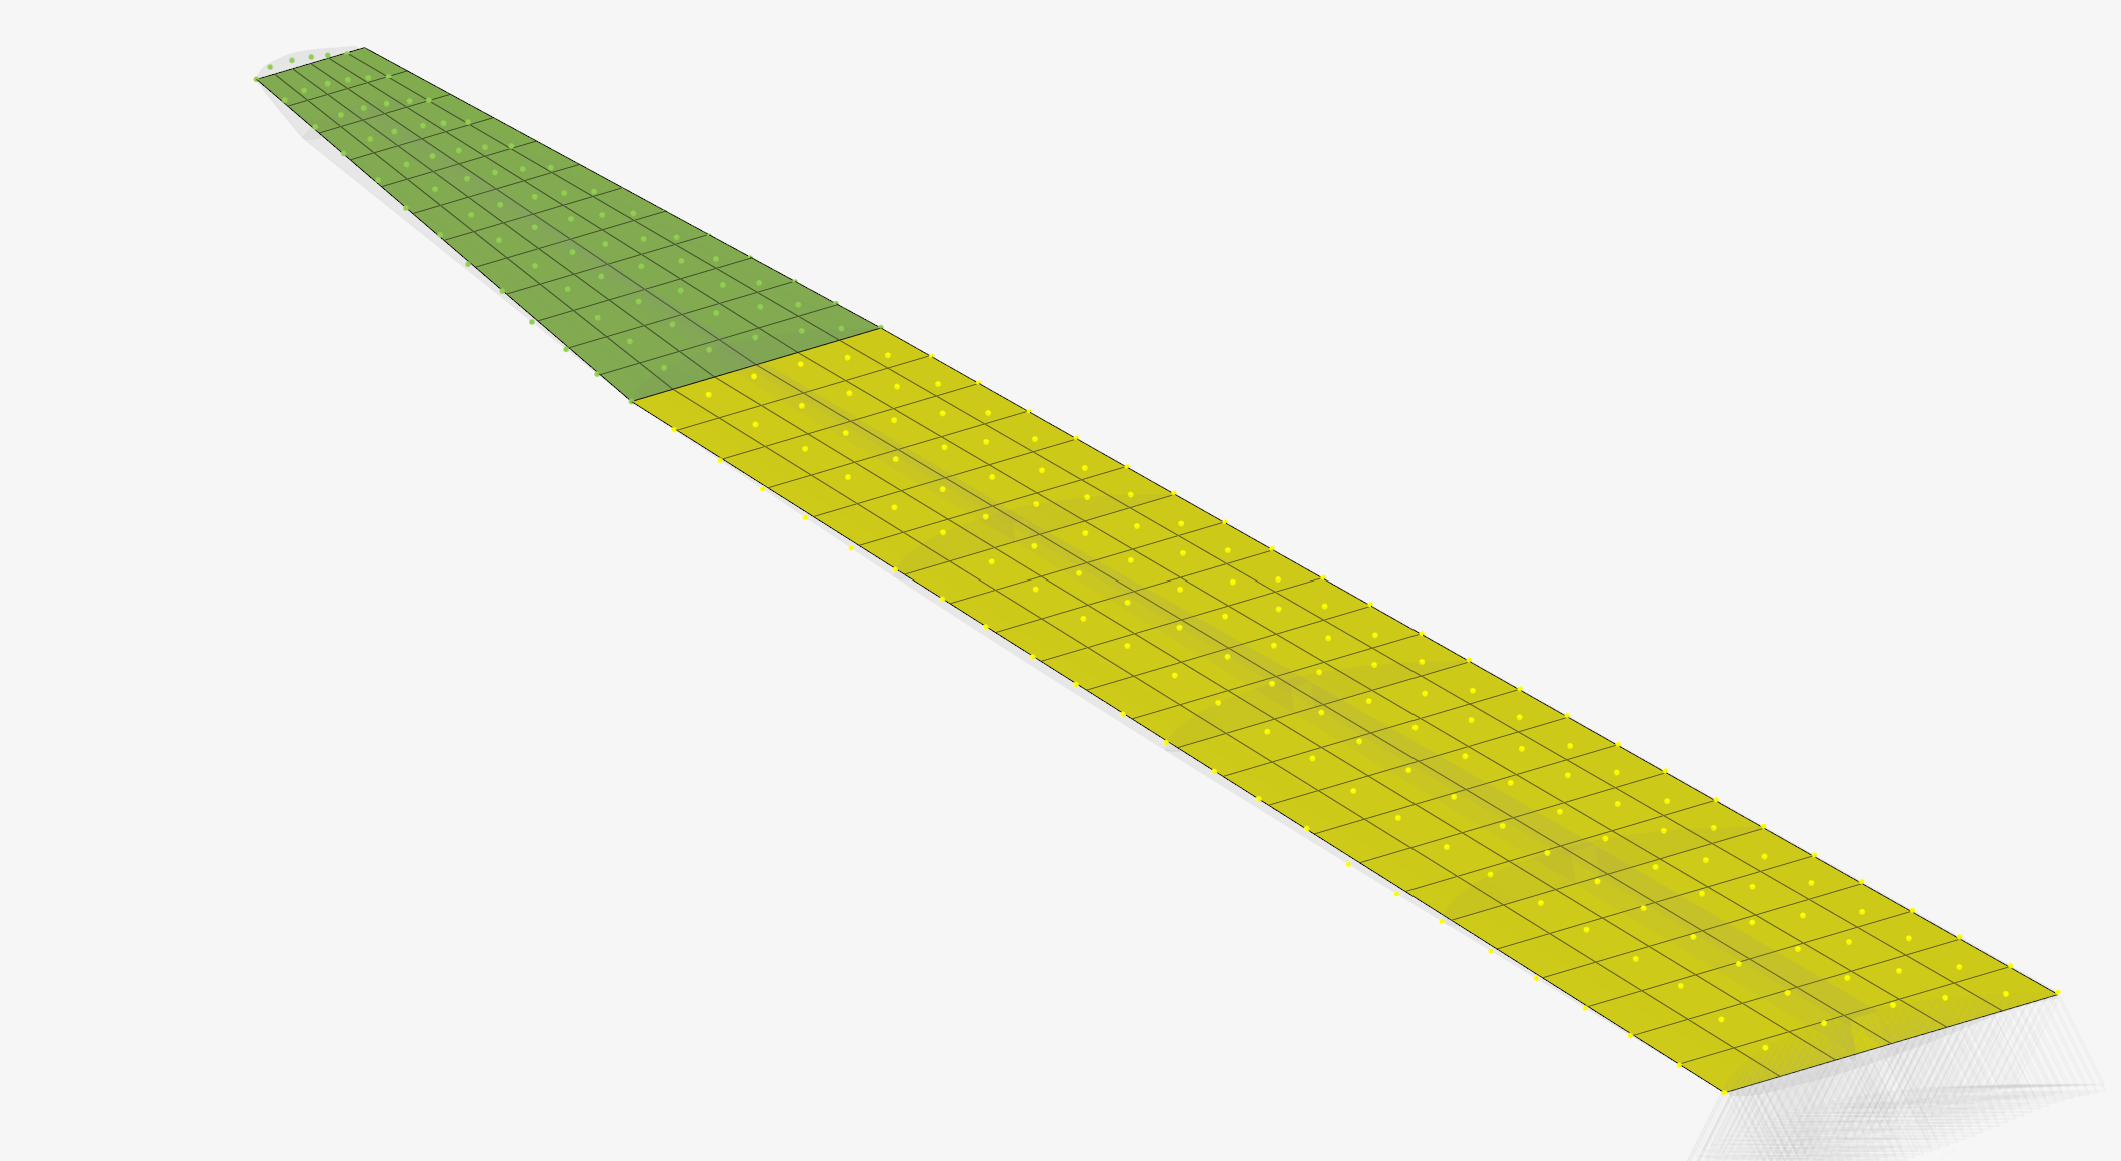
\includegraphics[width = \textwidth]{ASW 28 splines.png}
\caption{SPLINE1 entries of the ASW 28 Wing model}
\label{fig:SPLINE1}
\end{figure}

As can be seen in \autoref{fig:SPLINE1} two separate SPLINE1 entries were made in this model one for each CAERO entry defined previously. In this case nodes from the top surface of the wing are selected. The nodes are in series of along the span of the wing at various chord percentages, so as to closely match the aerodynamic grid points.

\subsection{Aeroelastic Problem Setup}
\label{aeroelastic-problem-setup}

To set up the Aeroelastic Flutter analysis several parameters need to be
defined.

\subsubsection{The AERO card:}

The AERO bulk data entry card defines basic parameters for dynamic
aeroelasticity regarding mainly the conditions of flight. The entries of
this card are summarized as follows:

\begin{itemize}
\item
  VELOCITY: has no effect for flutter analysis since the velocity
  varies during the analysis and defined elsewhere but cannot be left
  blank so unity is entered
\item
  REFC\textbf{:} Reference chord length used for the calculation of
  reduced frequency and lift and drag coefficients if requested
  \(REFC = 0.92m\)
\item
  RHOREF\textbf{:} Reference density \(RHOREF = 1.225\ kg\text{/}m^{3}\)
  which is the density of air at sea level
\item
  SYMXZ\textbf{:} which defines symmetry for the XZ plane and can have
  three values

  \begin{itemize}
  \item
    \textbf{-}1\textbf{:} for antisymmetry
  \item
    0: for no symmetry
  \item
    1: for symmetry
  \end{itemize}
\end{itemize}

\begin{quote}
for this application \(SYMZX\  = 1\)
\end{quote}

\begin{itemize}
\item
  \textbf{SYMXY:} defines symmetry for the XY plane in a similar way. In
  this analysis \(SYMXY = 0\)
\end{itemize}

\subsubsection{The MKAERO1 card:}

The MKAERO1 card is a bulk data entry card which is used to input a
table of Mach Numbers and Reduced Frequencies for which the aerodynamic
matrices are calculated.

The format of the MKAERO1 card has two column entries with a maximum of
eight elements each. One column is for the Mach number entry while the
other for the Reduced Frequencies. The aerodynamic matrices are computed
at every pair of values of reduced frequency and Mach number.

There are no concrete recommendations for the range of reduced
frequencies that must be covered by this entry, but since the
aerodynamic matrices are interpolated for the actual resultant reduced
frequency logic dictates that the range of reduced frequencies must be
at least greater than the resultant range of reduced frequencies. Of
course, this cannot be known a priori since the resultant reduced
frequencies are only made known after the analysis is run. For this
analysis quite a wide range of reduced frequencies was used after
consulting many examples of this type of analysis.

In case more than eight values are required for reduced frequency or
Mach number a second MKAERO1 entry can be made.

The values used are as follows:

\[\overrightarrow{M} = \begin{matrix}
0.0
\end{matrix},\ \ \overrightarrow{K} = \begin{bmatrix}
0.2 \\
0.4 \\
0.8 \\
1.6 \\
3.2 \\
6.4 \\
10 \\
14
\end{bmatrix}\]

As can be seen there is only one Mach number \(M = 0\) which means that
incompressible flow is assumed. The aerodynamic matrices are calculated
at every point \(\left( M_{i}, K_{j} \right)\)

\subsubsection{The FLFACT card:}

The FLFACT bulk data entry card is a card that specifies a series of
aerodynamic factors. These factors are used to define:

\begin{enumerate}
\def\labelenumi{\arabic{enumi}.}
\item
  Density ratios
\item
  Mach Numbers
\item
  Reduced Frequencies or Velocities (PK Method only).
\end{enumerate}

These factors can be defined using two different formats.

\begin{enumerate}
\def\labelenumi{\arabic{enumi}.}
\item
  In Format 1 a series of values is directly entered into the card
\item
  In Format 2 the so-called THRU format is used defining a series of
  values using:

  \begin{enumerate}
  \def\labelenumii{\alph{enumii}.}
  \item
    F1: The first factor
  \item
    FNF: the final factor
  \item
    NF: The Number of factors (integer)
  \item
    FMID: The intermediate aerodynamic factor
  \end{enumerate}
\end{enumerate}

The actual series of values produced when using the THRU format are
calculated using the following formula:

\begin{multline}
\frac{F1(FNF - FMID)(NF - i) + FNF(FMID - F1)(i - 1)}{(FNF - FMID)(NF - i) + (FMID - F1)(i - 1)}\\ ,where\ i = 1,2\ldots,NF
\end{multline}

Note that when \(FMID = \frac{F1 + FNF}{2}\) the factors are equally
distributed between F1 and FNF

For this Analysis three FLFACT Entries are needed:

\begin{itemize}
\item
  FLFACT 1: Is the density factor(s) and has a value of \(1\). This
  factor is multiplier of the Reference Density define in the AERO card
  and indicates that the analysis is to be performed at
  \(1 \times RHOREF\)
\item
  FLFACT 2: Is the Mach Number(s) and has a Value of \(0\). This factor
  is the Mach Number at which the analysis is to be performed.
\item
  FLFACT 3: Is the Velocity/ties at which the analysis is to be
  performed. This FLFACT is defined using the THRU Format with factors:

  \begin{itemize}
  \item
    \(F1\  = 20m/s\)
  \item
    \(FNF = 320m/s\)
  \item
    \(NF = 30\)
  \item
    \(FMID = 160\)
  \end{itemize}
\end{itemize}

The analysis is performed for every combination of combination of
density Mach number and velocity in the FLFACT entries

\subsubsection{The Flutter card:}

The flutter bulk data entry card specifies the method and parameters of
aeroelastic flutter analysis:

The most important fields of this card are

\begin{enumerate}
\def\labelenumi{\arabic{enumi}.}
\item
  METHOD the method can be one of K, PK, PKNL, KE for this analysis the
  PK method is used.
\item
  DENS: a reference to the FLFACT Bulk Data entry which specifies the
  density multipliers
\item
  MACH: a reference to the FLFACT Bulk Data entry which specifies the
  Mach number
\item
  VEL: a reference to the FLFACT Bulk Data entry which specifies the
  velocities
\item
  IMETH the interpolation method for the aerodynamic matrix which can be
  either L or S for linear or surface interpolation respectively. The
  default value of L is retained for this analysis
\end{enumerate}

\subsubsection{The EIGRL card:}

The EIGRL bulk data entry card defines the data required to perform real
eigenvalue analysis with the Lanczos method. The main fields of this
card are:

\begin{enumerate}
\def\labelenumi{\arabic{enumi}.}
\item
  V1, V2 Frequency range of analysis
\item
  ND Number of desired eigenfrequencies
\end{enumerate}

For this analysis, the Values \(V1 = 0.0\ Hz\) and \(ND = 8\) are used.
These values mean that the first eight eigenfrequencies starting from
zero Hertz will be calculated.

\subsubsection{Subcase Definition:}

For the subcase definition the ``Aerodynamic Flutter'' analysis type is
selected and then

\begin{itemize}
\item
  The FMETHOD field requires a reference to the Flutter card
\item
  The SPC Field requires a reference to the SPC load collector
\item
  The METHOD Field requires a reference to the EIGRL
\item
  The CMETHOD Field requires a reference to an EIGC card but can be left
  blank if no complex eigenvalues need to be computed (it is blank in
  this case since no structural damping is considered)
\item
  The SMETHOD Field requires a reference to a damping curve TDMP but can
  be left blank if structural damping is not considered. (it is blank in
  this case since no structural damping is considered)
\end{itemize}

The results of the aeroelastic flutter analysis are presented in \autoref{initial-flutter-analysis} 

\section{Optistruct -- Python Interface}\label{optistruct-python-interface}

\subsection{Results of Flutter Analysis \& Python }
\label{results-of-flutter-analysis-python}

The output of the analysis defined in the previous section is a .flt
text file in addition to the typical Optistruct .out output file. It has
a very specific format. It is organized in blocks of information each
corresponding to a different combination of Mach number, Density
(defined in the FLFACT entries) and Eigenmode number. The most important
aspects of the .flt file are outlined in \autoref{fig:Optistruct.fltfileexplanation} .

\begin{figure}[H]
    \centering
    \includesvg[width=\textwidth]{Flt file explanation.svg}
    \caption{Optistruct .flt file explanation}
    \label{fig:Optistruct.fltfileexplanation}
\end{figure}

The typical .out file, which is also output contains information about
whether the solver encountered any exceptions or warning and most
importantly information about the mass of the structure.

From the data contained in the .flt file two very useful plots can be
produced.

\begin{enumerate}
\def\labelenumi{\arabic{enumi}.}
\item
  The V-g plot plots the damping of each eigenmode (y-axis) against
  Velocity (x-axis)
\item
  The V-f plot plots the frequency of each eigenmode (y-axis) against
  Velocity (x-axis)
\end{enumerate}

\begin{figure}[H]
  \centering
  \begin{minipage}{0.495\textwidth}
      \centering
      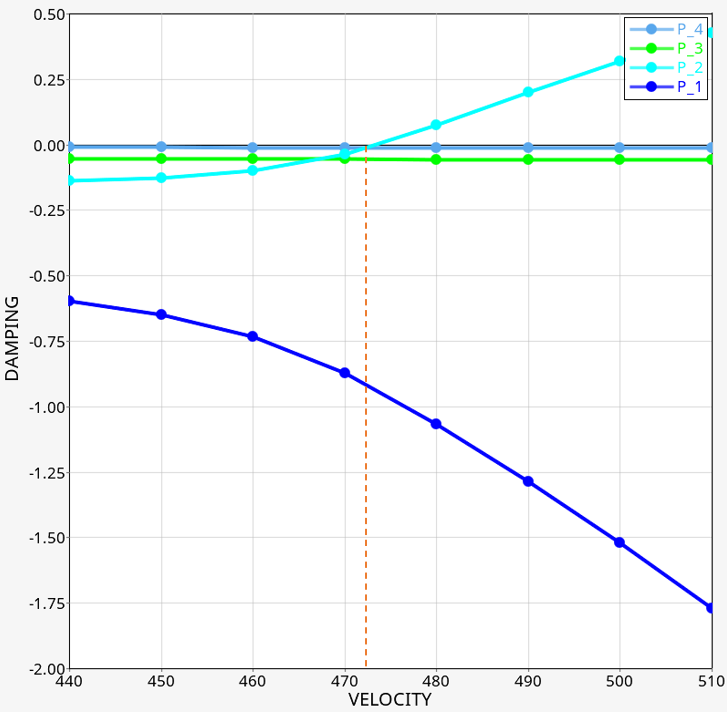
\includegraphics[width=\linewidth]{Example VG plot.png}
  \end{minipage}
  \hfill
  \begin{minipage}{0.495\textwidth}
      \centering
      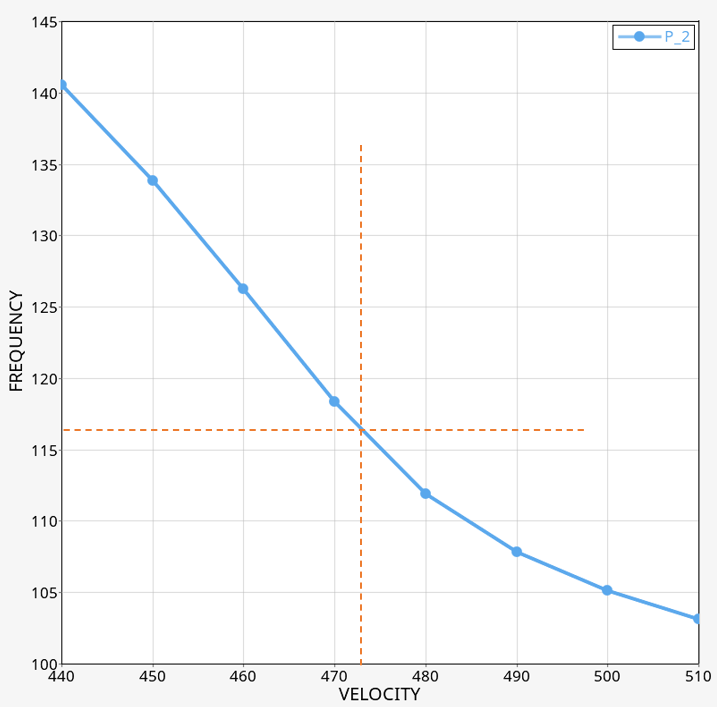
\includegraphics[width=\linewidth]{Example VF plot.png}

  \end{minipage}
  \caption{Example of V-g and V-f plot containing four eigenmodes \cite{altair_flutter_tips}}
\end{figure}


From these data one can determine the Flutter speed by examining the V-g
plot. More specifically a mode diverges when the damping of that
particular mode changes from negative to positive. Note that many modes
can diverge, but the flutter speed of the structure is determined by the
mode that diverges at the lowest speed.

The data blocks contained in the .flt file are read by a python script
and stored as pandas data frames. To determine the flutter velocity the
sign changes of each eigenmode are monitored until a negative to
positive change is detected. Then all the points where there is such a
sign change are stored and the flutter speed is determined by the
minimum speed at which such a sign change occurs.

A separate function is responsible for reading the .out file and
determining if the solver completed the analysis successfully as well as
recording the mass of the structure.

\subsection{Modifying Optistruct's input using
python}\label{modifying-optistructs-input-using-python}

In order to optimize the composite material of the structure one needs
to be able to modify the composite material's property programmatically
so that one can try many different variations and arrive at an optimum.
Optistruct makes this quite easy because it uses a text input file that
encodes all the information of the model. This file is called a .fem
file and can be output from HyperMesh as a comma separated text file. To
modify the composite material's property it is necessary to locate the
correct part of this file and decode it. According to Optistruct's
documentation the composite material's property is encoded in the
following way.

\begin{table}[h]
  \centering
  \resizebox{\linewidth}{!}{ % Fits table to page width
    \begin{tabular}{|c|c|c|c|c|c|c|c|c|c|}
      \hline
      1 & 2 & 3 & 4 & 5 & 6 & 7 & 8 & 9 & 10 \\ 
      \hline
      PCOMP & PID & Z0 & NSM & SB & FT & TREF & GE & LAM & + \\ 
      \hline
      & MID1 & T1 & THETA1 & SOUT1 & MID2 & T2 & THETA2 & SOUT2 & + \\ 
      \hline
      & MID3 & T3 & THETA3 & SOUT3 & Etc. & & & & \\ 
      \hline
    \end{tabular}
  }
  \caption{Table Fitted to Page Width}
\end{table}


Where:

\begin{itemize}
\item
  PCOMP: is the keyword indicating that a composite material property
  definition follows (string)
\item
  PID: is the ID of the property (integer)
\item
  NSM: is the non-structural mass per unit area (float)
\item
  SB: allowable inter lamina shear stress (default 0.0) (float)
\item
  FT: Failure Theory selection
\item
  TREF: Reference stress free temperature (float)
\item
  GE: Damping coefficient (float)
\item
  LAM: Laminate option different ways to define the laminate. In the
  default case all plies must be defined one by one
\item
  MIDi: The material ID of ply i (integer)
\item
  Ti: The thickness of ply i
\item
  THETAi: The angle of ply i
\item
  SOUTi: Stress, Strain output request default NO (bool)
\end{itemize}

The quantities to modify are mainly the Ti and THETAi entries to cover
the decision variables that will be needed.

\section{Optimization Problem}\label{optimization-problem}

In this chapter the implementation of the optimization algorithms
discussed in the theory \autoref{optimization-techniques} will be discussed.

\subsection{Applying Powell's method}\label{applying-powells-method}

This algorithm is implemented using SciPy's \cite{2020SciPy-NMeth} minimization
function by selecting the \emph{method = ``Powell''} optional argument.
In order to define the optimization problem some other important
parameters need to be defined.

\subsubsection{Decision Variables:}

The first step is the definition of the decision variables. These
variables consist of the thickness and angle of each layer in the
composite material. Since the composite laminate consists of six layers,
that would mean that 12 decision variables would have to be used.

Because of the computational time required though, some assumptions have
to be made in order to reduce the complexity of the optimization
problem. These assumptions are:

\begin{itemize}
\item
  The layers are antisymmetric.

This means that for every layer at height \(z_{k}\) with ply angle
\(\theta_{k}\) above the middle surface there exists an identical layer
with the opposite ply angle \(- \theta_{k}\) at height \(- z_{k}\) from
the middle surface


\begin{figure}[H]
    \centering
    \includesvg[width=0.7\textwidth]{Antisymmetric layers.svg}
    \caption{Antisymmetric layer configuration}
\end{figure}


This assumption reduces the number of decision variables for the ply
angles in half since from the original six independent variables only
three need to be defined for the six layered composite.
\([ \theta_{1},\ \ \theta_{2},\ \ \theta_{3}]\)

This assumption is reasonable since most composites are either symmetric
or anti symmetric in order to reduce the membrane - bending coupling
effects.


\item
  Each layer has the same thickness.

This assumption reduces the number of independent variables from six to
just one, since only one thickness \([t]\) needs to be
defined.

This assumption is also quite reasonable since during manufacturing of
composite parts every layer originates from the same spool of carbon
fiber which has an even thickness in its entirety.
\end{itemize}

These two assumptions lead to the final decision variables being:

\begin{equation}
\vec{\mathbf{x}}=[t,\theta_{1},\theta_{2},\theta_{3}]^{T}
\label{eq:descisionvars}
\end{equation}
\subsubsection{Objective function:}

Next the objective function is defined. Two different scenarios were
considered for the objective function.

\begin{itemize}
\item
  Scenario 1: The objective function considers the mass as well as the
  flutter velocity. The concept behind the formulation of this objective
  function is to be able to minimize the mass of the structure while
  maintaining a sufficient flutter speed. This would normally fall under
  the category of multi-objective optimization, but Powell's method
  doesn't allow for that, so a work around is used. The penalty method
  has to be employed, thus resulting in the following formulation.

\begin{equation}
    f_{obj}\left( \vec{\mathbf{x}} \right) =
    \begin{cases} 
        M, & V_{flutter} > V_{limit} \\
        M + P \cdot \left( V_{limit} - V_{flutter} \right), & V_{flutter} < V_{limit}
    \end{cases}
    \label{eq:objpowell1}
\end{equation}

\begin{quote}
Where:
\end{quote}

\begin{itemize}
\item
  \(M\): is the mass
\item
  \(P\): is a large constant called the penalty
\item
  \(V_{limit}\): is the limit below which the flutter speed of the wing
  is deemed unacceptably low
\item
  \(V_{flutter}\): is the resultant flutter speed from the Optistruct
  solver
\end{itemize}



This definition allows for the minimization of mass while keeping the flutter speed above a certain limit. If the flutter speed drops below the specified limit a penalty term proportional to the amount by which the constraint is violated is added to the objective function so that the optimization algorithm is forced to return to a region where the
constraint is not violated any more.


\item
  Scenario 2: The simpler scenario is an objective function where the
  input is the decision variable vector from equation \eqref{eq:descisionvars} but
  excluding the thickness \(t\), and the output is the negated flutter
  velocity calculated by the Optistruct solver.


\begin{equation}
f_{obj}\left( \vec{\mathbf{x}} \right) = - V_{flutter},\ \ with\ \vec{\mathbf{x}}\mathbf{=}\left\lbrack \theta_{1},\theta_{2},\theta_{3} \right\rbrack^{T}
\label{eq:objpowell2}
\end{equation}

The negative sign on the velocity is so that minimization occurs in the direction of increasing flutter velocity. Also notice that thickness has been removed from the optimization variables. Since mass is not considered in the objective function the optimizer could simply increase the thickness of the material and achieve a higher flutter speed this way. This behavior is of course undesirable and is the reason why thickness was removed from the optimization variables and now remains constant throughout the optimization process along with the mass of the wing.
\end{itemize}

\subsubsection{Search space boundaries}

To fully define the optimization problem, the search space needs to be fully defined. The boundary definition is quite simple in this case.

\begin{itemize}
\item
  For Scenario 1:\\
  The thickness has to be restrained in addition to the angles. The boundaries for the thickness are defined to be within a reasonable range
  of 0.1 to 1 mm per layer.

\begin{equation}
\theta_{1},\theta_{2},\theta_{3} \in [ - 90^{o}, + 90^{o} ]
\end{equation}


\item
  For Scenario 2:\\
  Only the angles need to be constrained between -90 and +90 degrees so
  the constraints are:



\begin{equation}
t \in [ 10^{- 4},\ 10^{- 3} ]\quad and \quad \theta_{1},\theta_{2},\theta_{3} \in [ - 90^{o}, + 90^{o} ]
\end{equation}
\end{itemize}



\subsubsection{Acceleration of the algorithm}
Because of the computationally intensive nature of the objective function a way to reduce computational time was applied. Instead of the algorithm being able to choose any arbitrary floating-point number within the specified range of each optimization variable a slight compromise was made. The values of each variable are internally rounded to a specified precision given by the user. Moreover, the results of each iteration are stored in a cache so that in case the algorithm finds itself trying to use the same input, the calculations are omitted and the cached results is used instead. The caching in combination with the rounding result in far fewer calls to the Optistruct solver than would be otherwise required. In this application the angles are rounded to the nearest integer while the thickness is rounded to the nearest tenth of a
millimetre.

To illustrate this concept more clearly an example will be made:\\

Let's assume that the initial vector is
\({\vec{x}}_{0} = \lbrack 0.0005,\ \ 45,\  - 45,\ 45\rbrack^{T}\)

\begin{enumerate}
\def\labelenumi{\arabic{enumi}.}
\item
  For the first iteration let's assume that the algorithm tries


\[{\vec{x}}_{1} = \lbrack 0.00043,\  - 20.3,\  - 69.6\ ,\ 42.14\rbrack^{T}\]

this will internally get rounded to

\[{\vec{x}}_{1} = \lbrack 0.0004,\ \ 20,\  - 70,\ 42\rbrack^{T}\]

and the result will be cached

\item
  If in the second iteration the algorithm tries
\end{enumerate}

\[{\vec{x}}_{2} = \lbrack 0.00041,\  - 20.4,\  - 69.8\ ,\ 42.47\rbrack^{T}\]

it will still get rounded to

\[{\vec{x}}_{2} = \lbrack 0.0004,\ \ 20,\  - 70,\ 42\rbrack^{T}\]

and the same cached result will be used

The results of Powell's method are presented in \autoref{powells-optimization-method}


\subsubsection{Applying the Genetic Algorithm}
\label{applying-the-genetic-algorithm}

For the application of the genetic algorithm the PyGAD \cite{gad2023pygad} library
is used. In order to define the optimization problem for the genetic
algorithm many parameters need to be defined. Unfortunately, there is no
way of finding the optimal settings for every variable in every specific
problem. Therefore, the parameters were chosen after some
experimentation using a smaller number of generations which can be run
faster. The parameters that are selected are most probably not the most
optimal but work well enough.

\begin{enumerate}
\def\labelenumi{\arabic{enumi}.}
\item
  First and foremost, the \textbf{genes} and the \textbf{gene}
  \textbf{space} must be decided.

The genes are analogous to the optimization variables of classical
optimization algorithms and are chosen to be the three angles and the
thickness of the layers so four genes in total.

A range of possible values needs to be defined for every gene. The range
for every angle gene is:

\[\vartheta_{RANGE} = \lbrack - 90,\  + 90,\ step = 1\rbrack\]

and for the thickness:

\[t_{RANGE} = \lbrack 0.0001,\ 0.001,\ step = 0.0001\rbrack\]

these ranges define the gene space.

\item
  The so-called fitness function needs to be defined. The fitness
  function is analogous to the objective function of classical
  optimization algorithms. Because of the advanced abilities of this
  algorithm a multi-objective optimization is carried out where the two
  goals are:

  \begin{itemize}
  \item
    The minimization of the mass of the ASW 28 Wing structure
  \item
    The maximization of the Flutter Velocity.To achieve those goals a
    function is created with the following format
  \end{itemize}

\begin{equation}
f_{fitness}\left( \begin{bmatrix}
t \\
\vartheta_{1} \\
\vartheta_{2} \\
\vartheta_{3}
\end{bmatrix} \right)\  = \begin{bmatrix}
 - Mass \\
V_{flutter}
\end{bmatrix}
\end{equation}


The negative sign for the mass is because this algorithm works on
maximizing the fitness function.
\end{enumerate}


After those basic and mandatory inputs are defined, several other
parameters which control the way the algorithm runs are defined.


\begin{itemize}
\item
  \emph{Num\_generations = 1000, controls} the number of generations in
  the span of which evolution will take place. This parameter is chosen
  so that a reasonable computational time is maintained
\item
  \emph{sol\_per\_pop = 10,} the number of solutions that will be
  produced (number of chromosomes) after each generation
\item
  \emph{parent\_selection\_type = steady state selection}
\item
  \emph{keep\_elitisism = 4} which means that the four best solution of
  each generation are carried over to the next
\item
  \emph{crossover\_type = ``single point''}
\item
  \emph{crossover\_probability = 0.7} The probability of selecting a
  parent for applying the crossover operation. For each parent, a random
  value between 0.0 and 1.0 is generated. If this random value is less
  than or equal to the value assigned to the crossover\_probability
  parameter, then the parent is selected.
\item
  \emph{mutation\_type = ``random''}
\item
  \emph{mutation\_probability = 0.1} The probability of selecting a gene
  for applying the mutation operation. For each gene in a solution, a
  random value between 0.0 and 1.0 is generated. If this random value is
  less than or equal to the value assigned to the mutation\_probability
  parameter, then the gene is selected
\item
  \emph{mutation\_by\_replacement = True,} means replace the gene by the
  randomly generated value instead of adding the random value to it.
\end{itemize}

The results of the Genetic Algorithm are presented in \autoref{genetic-algorithm-optimization}


\subsection{Flutter Speed Prediction using Neural networks}
\label{flutter-speed-prediction-using-neural-networks}

The purpose of this section is to develop a surrogate model using Neural
Networks in order to potentially accelerate the process of optimization.
Surrogate models are often used in engineering when the outcome of
interest is not easily measured or when the computational effort
required for proper simulation is too great. The development of the
Neural Network models is done in python using the Keras library from
Tensorflow.

The development of neural networks is a multistep process.

\begin{enumerate}
\def\labelenumi{\arabic{enumi}.}
\item
  The training data for the models have to be collected and organized in
  a convenient way
\item
  The structure of the model and its parameters have to be defined
\item
  The model has to be trained on the training data
\item
  Lastly the performance of the network has to be evaluated
\end{enumerate}


\subsubsection{Training Data}

To acquire the training data the solver is run repeatedly for random
material parameters within specified ranges. The parameters that vary
are the same as those used for the optimization.

More specifically those parameters are:

The angle of the major axis of each layer assuming an antisymmetric
construction

\begin{equation}
\theta_{i} \quad \in [ - 90^{o}, + 90^{o}], \quad for\ i = 1,2,3
\end{equation}


The thickness of each layer assuming all the layers have equal thickness

\begin{equation}
t \quad \in [ 0.1, 0.9]\ mm
\end{equation}

3000 random datapoints were collected and organized in a data frame
where every row represents a data point and contains information about
the input variables used and the predicted flutter speed from Optistruct
which is the target variable of the Neural Network. The mass of the wing
was also recorded but this is not a target variable for the neural
networks that are about to be developed because the mass is directly
proportional to the thickness of the layers. \(Mass \propto t\). The
computational time required to gather all the data is approximately 23
hours.


\subsubsection{Model Structure \& parameters}

The structure of the layers is a very important aspect of neural
networks. There is no way to know a priori the optimal structure of the
neural network so that a good prediction is made, and a reasonable
training time is achieved. For this reason, many different models will
be created, and their performance will be evaluated in order to find the
best one.

The first layer of every Neural Network is a normalization layer. This
is an important step that ensures a consistent scale between the
different data types of the input. In turn this ensures that no feature
dominates the learning process. Furthermore, normalization can improve
convergence by keeping the weights and activations within a reasonable
range. Lastly normalization can help by reducing the overfitting and
making a model more robust.

For this example, the two different kinds of inputs (the angles and the
thickness) have very different ranges since the angles vary between -90
and +90 while the thicknesses are four orders of magnitude smaller
varying between 0.0001 and 0.001 meters.

The normalization layer in Keras shifts and scales the input data into a
distribution centered around 0 and with a standard deviation of 1 by
subtracting the mean of the training data and the dividing by the square
root of the variance in the data.

\begin{equation}
f_{norm}(x) = \frac{x - mean\left( \overrightarrow{x} \right)}{\sqrt{var\left( \overrightarrow{x} \right)}}
\end{equation}

The mean and variation of the data is calculated based on the training
data. If the training data is not representative of the actual data on
which the network will be called to make predictions on, the
normalization might fail producing a non-centered distribution with a
variation much different than 1.

After the normalization layer the hidden layers follow. These layers
differ in number from model to model. In this work Neural Networks with
1, 2, 4, and 6 hidden layers will be tested. Each layer has 64 Neurons
and uses the RELU activation function.

Finally the output layer is added which uses a linear activation function
as this is a regression problem and only has 1 Neuron because the only
prediction that these neural networks make is the flutter speed of the
ASW 28 Wing model.

\begin{figure}[H]
  \centering
  \begin{minipage}{0.4\textwidth}
      \centering
      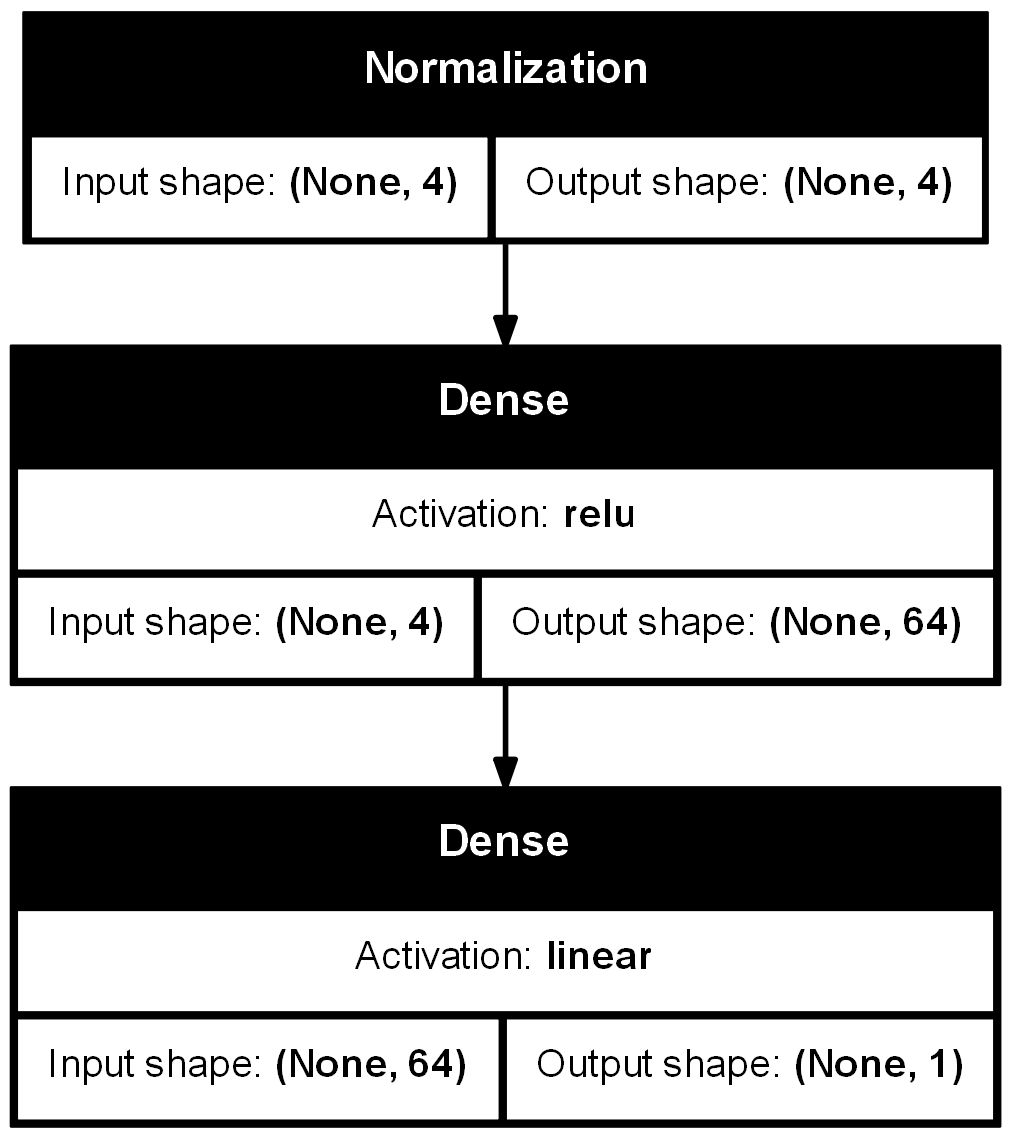
\includegraphics[width=\linewidth]{images/Results/Neural Net/1HL/structure.png}
      \caption{Neural Network Structure with $1$ Hidden layer}
  \end{minipage}
  \hfill
  \begin{minipage}{0.4\textwidth}
      \centering
      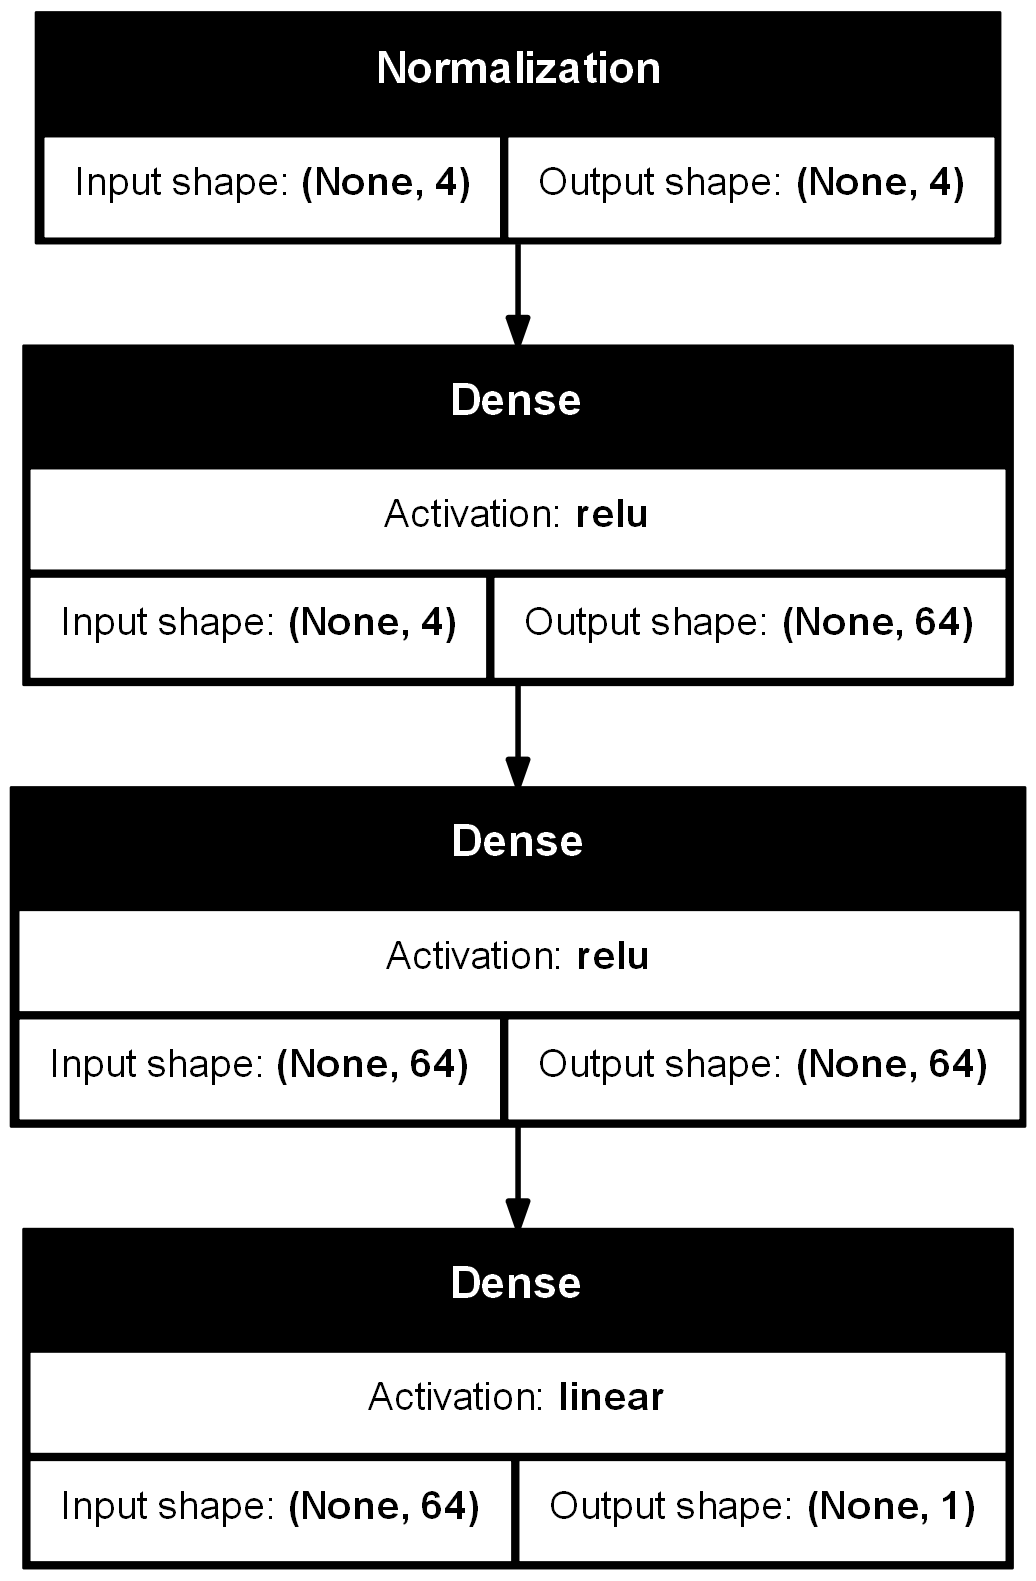
\includegraphics[width=\linewidth]{images/Results/Neural Net/2HL/structure.png}
      \caption{Neural Network Structure with $2$ Hidden layer}


  \end{minipage}
\end{figure}

\begin{figure}[H]
  \centering
  \begin{minipage}{0.4\textwidth}
      \centering
      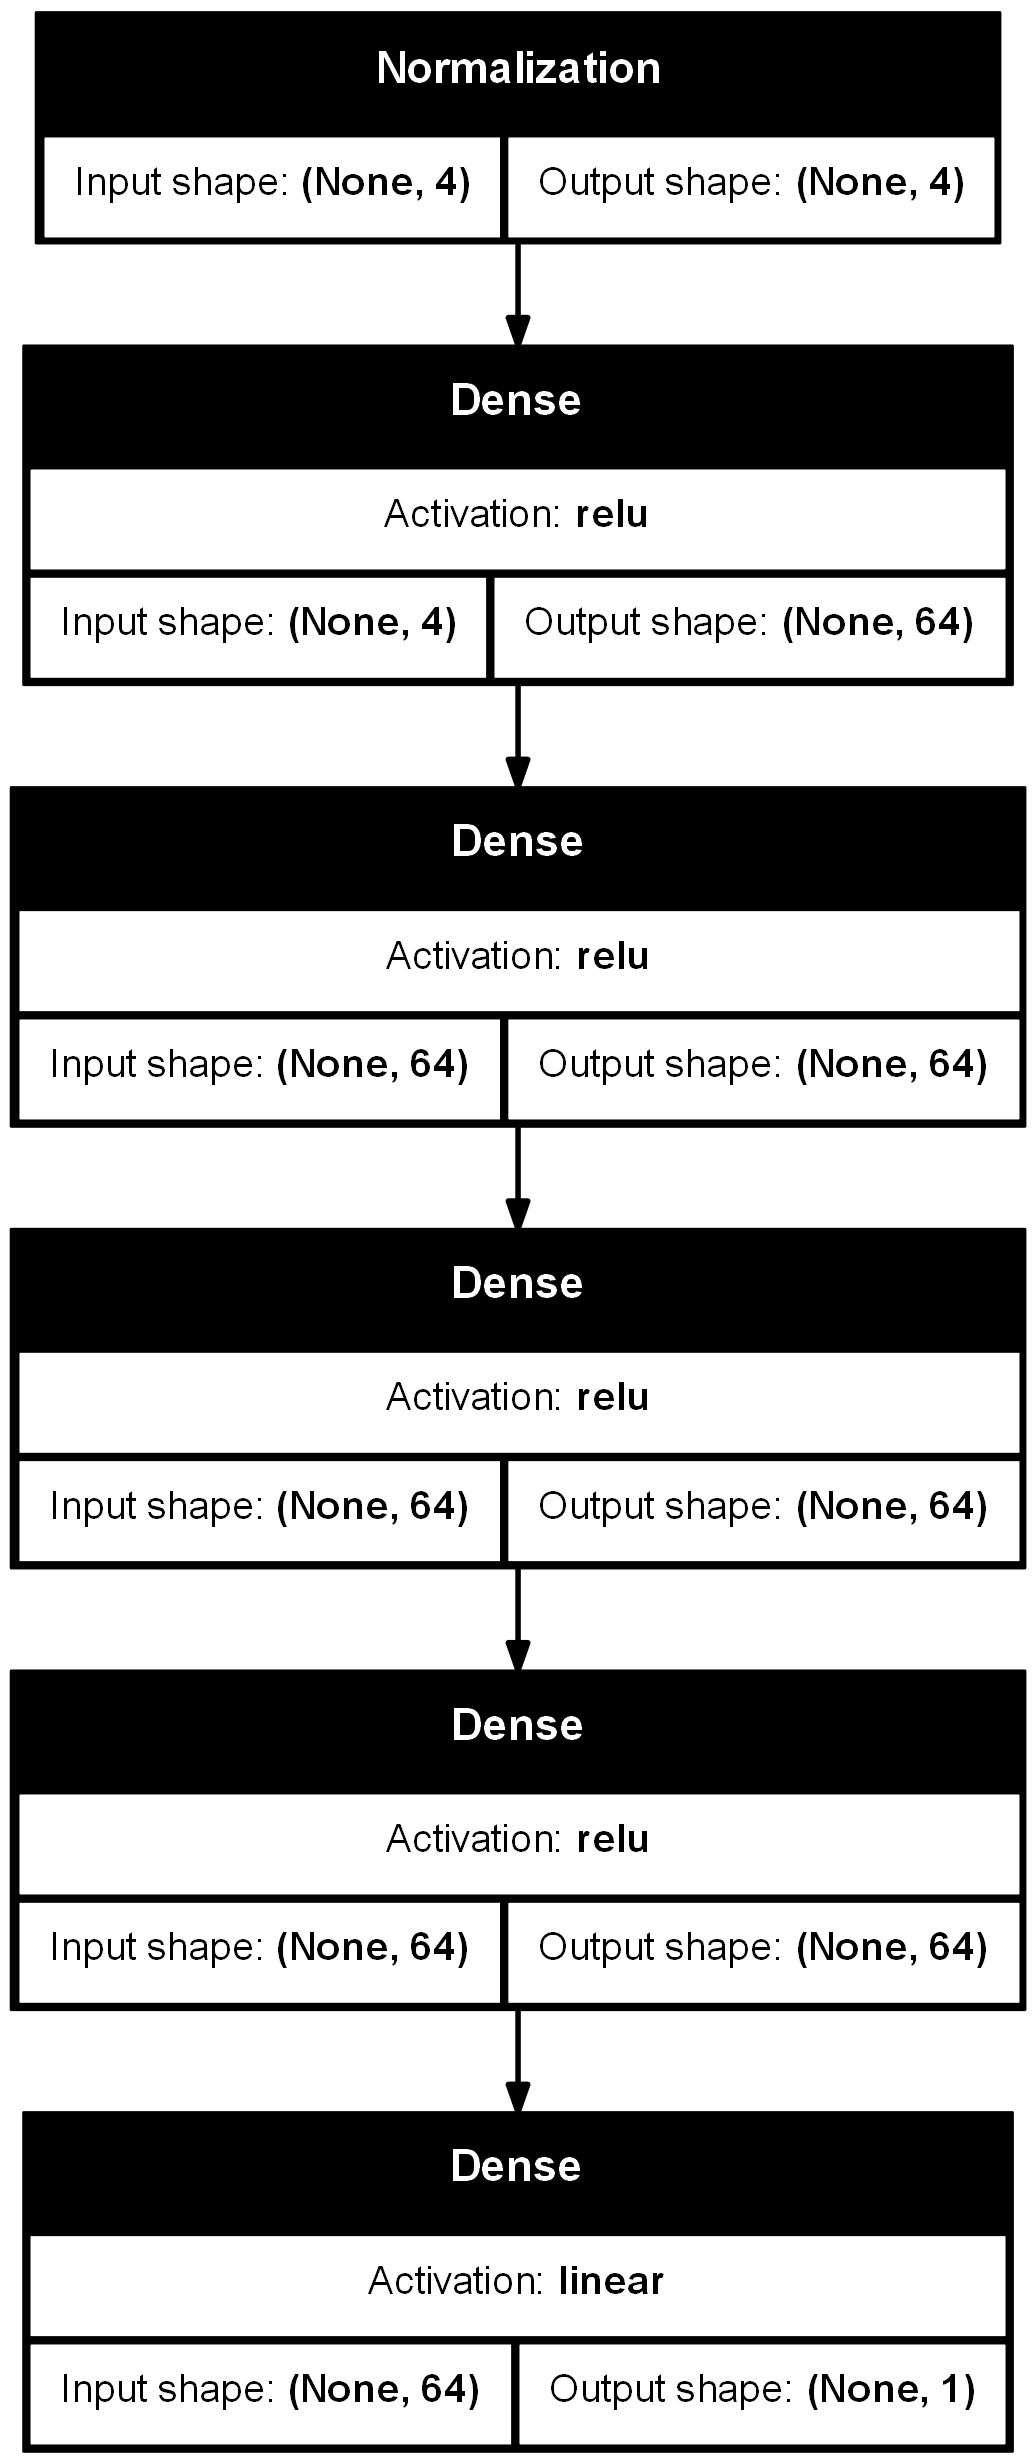
\includegraphics[width=\linewidth]{images/Results/Neural Net/4HL/structure.png}
      \caption{Neural Network Structure with $4$ Hidden layer}
  \end{minipage}
  \hfill
  \begin{minipage}{0.4\textwidth}
      \centering
      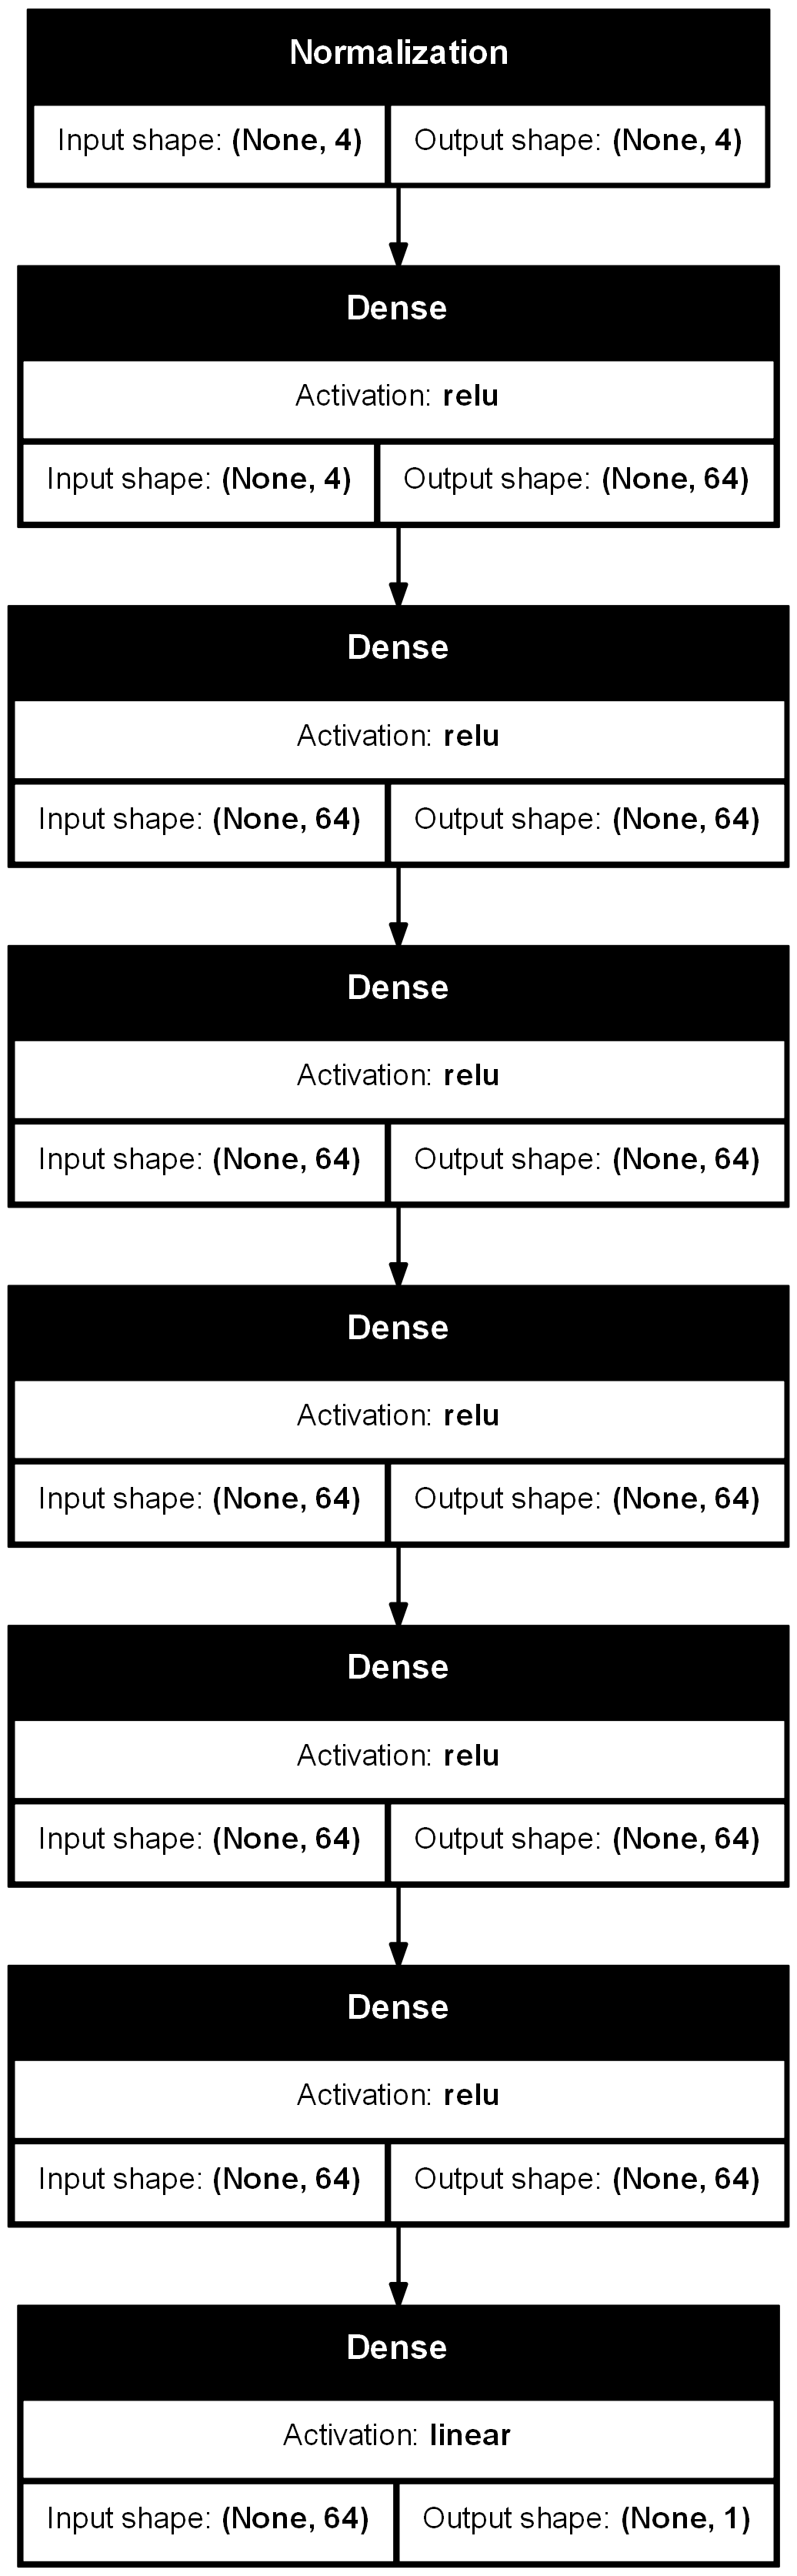
\includegraphics[width=\linewidth]{images/Results/Neural Net/6HL/structure.png}
      \caption{Neural Network Structure with $6$ Hidden layer}
  \end{minipage}
\end{figure}


\subsubsection{Loss Function}

The loss function of choice for this application is the Mean Average
Error described in \autoref{eq:MAE} because it is easy to
interpret as it has the same units as the output variable and is robust
to outliers.

\subsubsection{Optimizer}

The optimizer of choice is Adam which is widely used and considered one
of the best optimizers with a learning rate of 0.01

\subsubsection{Hyper Parameter Tuning}
\label{Hyper-Parameter-Tuning}

Finally, a Hyper tuned model is constructed using the HyperBand
Algorithm. The model is free to choose the following hyperparameters:

\begin{itemize}
\item
  The Number of Hidden layers between 1 and 10
\item
  The number of Neurons for each layer from a discrete set of values
  \[\left\{ 2^{i} \right\}, \ with\ i = 1,2,\ldots ,10\]
\item
  The activation function of each layer with the choices being ReLu,
  tanh, Leaky ReLu
\item
  The learning rate of the optimizer
\end{itemize}

The structure of this model is not known at this phase as it is a
product of the optimization process. This is why it will be presented in
the results section.

The results of the Neural networks are presented in \autoref{neural-network-prediction-results}